%%%  Template to prepare a defense of Bc./Mgr./... thesis
%%%  to be presented at MFF
%%%  (unofficial)
%%%
%%%  AUTHOR:  Arnošt Komárek
%%%           Department of Probability and Mathematical Statistics
%%%           Faculty of Mathematics and Physics, Charles University in Prague
%%%
%%%  LOG:    20150505  created by modification of some previous personal presentations
%%%          20170522  update related to new MFF logo
%%%  
%%%  ===========================================================================
\documentclass[c, 10pt]{beamer}


%%%%% Package needed if some accented letters in the presentation
%%%%% -------------------------------------------------------------
\usepackage[utf8]{inputenc}



\usepackage{pgf,tikz,pgfplots}
\pgfplotsset{compat=1.15}
\usepackage{mathrsfs}
\usetikzlibrary{arrows}
\usepackage{enumerate}


\usepackage{ulem} % \sout strikethrough




%%%%% Most beamer settings and other LaTeX commands
%%%%% are provided in the file below
%%%%% -----------------------------------------------------
%%%
%%%  Style for MFF related presentations
%%%  (unofficial)
%%%
%%%  AUTHOR:  Arnošt Komárek
%%%           Department of Probability and Mathematical Statistics
%%%           Faculty of Mathematics and Physics, Charles University in Prague
%%%
%%%  LOG:    20150430  created by modification of some previous personal presentations
%%%          20170522  modified (new MFF logo)
%%%  
%%%  ===========================================================================

%%%%% If to determine whether Czech or English version
%%%%% of a presentation is to be produced
%%%%% default = Czech
%%%%% ------------------------------------------------------
\newif\ifCZversion
\CZversiontrue

\ifCZversion\else\renewcommand{\uv}[1]{``#1''}\fi


%%%%% Included packages
%%%%% ----------------------------------------------------------
\usepackage{helvet}                       % font
\usepackage{amsmath, amssymb}
\usepackage{delarray}
\usepackage{multicol}
\usepackage{graphicx, fancybox}
\usepackage{psfrag}
\usepackage{fancyvrb}
\usepackage{eurosym}
\usepackage{bbding}
%\usepackage{marvosym}
\usepackage{wasysym}
\usepackage[czech]{babel}
\usepackage{mathrsfs}
\usepackage[pdftex]{bookmark}

\usepackage{bbm}	% For lowercase blackboard bold
\usepackage{multicol}  	% ultiple columns
\usepackage{enumerate}

%%%%% Some LaTeX commands
%%%%% ----------------------------------------------------------
\renewcommand{\arraystretch}{1.2}


%%%%% Some colors and related commands
%%%%% ----------------------------------------------------------

  %% Pantone 186 = "official" red of MFF
\definecolor{redmff}{rgb}{0.7892720,0.0651341,0.1455939}          

  %% First level color = black
\definecolor{colOne}{rgb}{0,0,0}
\newcommand{\tOne}[1]{\textcolor{colOne}{#1}}
\newcommand{\tOneb}[1]{\textcolor{colOne}{\textbf{#1}}}
\newcommand{\tOnei}[1]{\textcolor{colOne}{\textit{#1}}}

  %% Second level color = quite dark blue
\definecolor{colTwo}{rgb}{0,0,0.3}                
\newcommand{\tTwo}[1]{\textcolor{colTwo}{#1}}
\newcommand{\tTwob}[1]{\textcolor{colTwo}{\textbf{#1}}}
\newcommand{\tTwoi}[1]{\textcolor{colTwo}{\textit{#1}}}

  %% Third level color = something between blue3 and blue4
\definecolor{colThree}{rgb}{0,0,0.7}              
\newcommand{\tThree}[1]{\textcolor{colThree}{#1}}
\newcommand{\tThreeb}[1]{\textcolor{colThree}{\textbf{#1}}}
\newcommand{\tThreei}[1]{\textcolor{colThree}{\textit{#1}}}

  %% Color to alert (highlight) = MFF red
\definecolor{alertCol}{rgb}{0.7892720,0.0651341,0.1455939}
\newcommand{\tal}[1]{\alert{#1}}
\newcommand{\talb}[1]{\textbf{\alert{#1}}}
\newcommand{\tali}[1]{\textit{\alert{#1}}}

  %% White
\newcommand{\tw}[1]{\textcolor{white}{#1}}
\newcommand{\twb}[1]{\textcolor{white}{\textbf{#1}}}
\newcommand{\twi}[1]{\textcolor{white}{\textit{#1}}}

  %% Some other colors used somewhere
\definecolor{semiwhite}{gray}{0.98}
\definecolor{mffgray}{gray}{0.95}
\definecolor{semiblack}{gray}{0.5}
\definecolor{rred}{rgb}{0.5,0,0}


%%%%% Beamer stuff
%%%%% ----------------------------------------------------------
\mode<presentation> {

    %%% General theme of a presentation (some pre-specified themes)
    %%% ------------------------------------------------------------------
    %\usetheme{CambridgeUS}
    \usetheme{Warsaw}

    %%% Color schemes that will be used unless redefined below
    %%% ------------------------------------------------------------------
    %\usecolortheme{wolverine}
    \usecolortheme{beaver}


    %%% Color schemes for different elements of a presentation
    %%% ---------------------------------------------------------

      %%% Uncomment the two rows below if some background file (layout) is to be used
      %%% on all slides
    %\usebackgroundtemplate{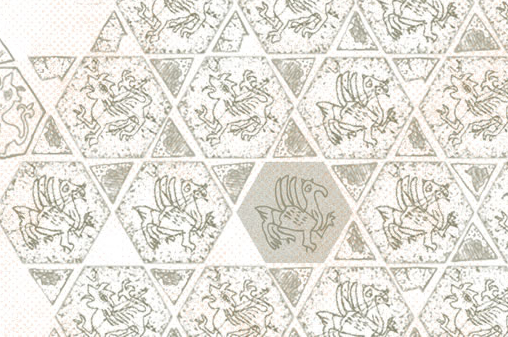
\includegraphics[width=\paperwidth, height=\paperheight]{./FigureLayout/BackgroundRotunda}}
    %\setbeamercolor{background canvas}{bg=}                                                             

      %%% Setting for "standard" slides
      %%% - must be commented if background file used
    \setbeamertemplate{background canvas}[vertical shading][bottom=semiwhite, top=white, middle=semiwhite!50!white]
    \setbeamercolor{background canvas}{bg=white}                           %% NO EFFECT WHEN \setbeamertemplate{background canvas} WAS USED

      %%% Colors of frametitle, normal, alerted and math texts
    \setbeamercolor{frametitle}{fg=white, bg=redmff}
    \setbeamercolor{normal text}{fg=black}
    \setbeamercolor{alerted text}{fg=redmff}
    \setbeamercolor{math text inlined}{fg=colTwo}
    \setbeamercolor{math text displayed}{fg=colTwo}

      %%% Colors for some special boxes defined below
    \setbeamercolor{mffboxcol}{fg=colTwo, bg=mffgray}
    \setbeamercolor{mffboxcolupper}{fg=white, bg=redmff}

    %%% Set serif font (patkové písmo) in mathematics
    %%% ------------------------------------------------
    %\usefonttheme[onlymath]{serif}

    %%% Itemize style (rectangles instead of bullets)
    %%% ------------------------------------------------
    % \useinnertheme{rectangles}

    %%% Default content of a header of each slide
    %%% (currently nothing)
    %%% ------------------------------------------------
    \setbeamertemplate{headline}{}

    %%% Default content of a foot of each slide
    %%% ------------------------------------------------
    %\setbeamercolor{page number in head/foot}{fg=black, bg=white}
    \setbeamertemplate{footline}{
      \hspace*{2.5em}
      \begin{beamercolorbox}{section in head/foot}
      \vskip1pt
      \tOne{\rule{\textwidth}{1pt}}
      \vskip2pt

      %%% Foot containing (a) page number/total number of pages, (b) name, (c) short title of presentation
      {\small \tOne{\insertframenumber}\textcolor{semiblack}{/\inserttotalframenumber}}\hspace{1em}
      \tOne{\footnotesize \insertauthor}\hfill
      \textcolor{redmff}{\footnotesize\insertshorttitle\hspace{3em}}

      %%% Foot containing (a) page number/total number of pages, (b) name, (c) short section title
      %{\small \tOne{\insertframenumber}\textcolor{semiblack}{/\inserttotalframenumber}}\hspace{1em}
      %\tOne{\footnotesize \insertauthor}\hfill
      %\textcolor{redmff}{\footnotesize\thesection. \insertsection\hspace{3em}}
    
      \hspace*{3.5em}
      \vskip3pt
      \end{beamercolorbox}
    }

    %%% Title page
    %%% -------------------
    \setbeamertemplate{title page}{
      %\vspace*{-0.5em}
      \begin{center}
      \textcolor{black}{\normalsize\bfseries\rmfamily \insertinstitute}

      \vspace{1em}
        
      \ifCZversion
        
\includegraphics[width=0.8\textwidth]{./FigureLayout/mff_cz_color}
      \else
        
\includegraphics[width=0.8\textwidth]{./FigureLayout/mff_en_color}
      \fi

      \medskip
      \noindent\textcolor{redmff}{\rule{\textwidth}{2pt}}
  
      \bigskip
      \textcolor{black}{\normalsize\bfseries \insertauthor} \\[0.5ex]

      \bigskip
      \textcolor{redmff}{\Large\bfseries \inserttitle}

      \medskip
      \textcolor{redmff}{\large\insertsubtitle}

      \medskip
      \noindent\textcolor{redmff}{\rule{\textwidth}{2pt}}
      
      \medskip
      \textcolor{colTwo}{\small \insertdate}
      \end{center}
    }    

    %%% Switch-off/on foot with navigation symbols    
    %%% -----------------------------------------------
    % \setbeamertemplate{navigation symbols}{}
    \usenavigationsymbolstemplate{}

    %%% Left and right margin
    %%% --------------------------------
    %\setbeamersize{text margin left=1cm}
    %\setbeamersize{text margin right=1cm}


    %%% Use of a logo on each slide
    %%% (not really recommended, so commented)
    %\logo{
\includegraphics[height=1.5cm, width=1.5cm]{./FigureLayout/mff_logo}}
}


%%%%% Commands to produce slides at the beginning of each section
%%%%% --------------------------------------------------------------
\renewcommand{\thesection}{\arabic{section}}
\newcommand{\framesection}{
  \begin{frame}%[plain]

  \vspace*{2em}
  \begin{center}\Large
  \ifCZversion Oddíl \thesection \else Section \thesection \fi
  \end{center}

  \begin{center}\color{rred}\Large
  \insertsection
  \end{center}

  \end{frame}
}


%%%%% Style for software related stuff
%%%%% ----------------------------------------------------------
\newcommand{\Rko}{
\includegraphics[width=5.094mm, height=3.876mm]{./FigureLayout/Rlogo}}
\newcommand{\Rfun}[1]{\textcolor{redmff}{\texttt{#1}}}

\DefineVerbatimEnvironment{Rin}{Verbatim}{formatcom=\color{redmff}, fontsize=\scriptsize, frame=single, framerule=1pt, framesep=2pt}
\DefineVerbatimEnvironment{Rout}{Verbatim}{formatcom=\color{blue}, fontsize=\scriptsize, frame=single, framerule=1pt, framesep=2pt}


%%%%% Boxes
%%%%% ----------------------------------------------------------
\newcommand{\mffbox}[2][0pt]{%
  \begin{beamercolorbox}[center, sep=#1, rounded=true, shadow=true]{mffboxcol}
  #2
  \end{beamercolorbox}
}

\newcommand{\mffboxTitle}[2]{%
  \begin{beamerboxesrounded}[lower=mffboxcol, upper=mffboxcolupper, shadow=true]{#1}
  #2
  \end{beamerboxesrounded}
}


%%%%% Some constructions for displayed math
%%%%% ----------------------------------------------------------
\newcommand{\dmath}[2][-1.4em]{%
  \begin{beamercolorbox}[center, sep=#1, rounded=true, shadow=true]{mffboxcol}
  \begin{displaymath}
  #2
  \end{displaymath}
  \end{beamercolorbox}
}

\newcommand{\dalign}[2][-1.4em]{%
  \begin{beamercolorbox}[center, sep=#1, rounded=true, shadow=true]{mffboxcol}
  \begin{align*}
  #2
  \end{align*}
  \end{beamercolorbox}
}

\newcommand{\dgather}[2][-1.4em]{%
  \begin{beamercolorbox}[center, sep=#1, rounded=true, shadow=true]{mffboxcol}
  \begin{gather*}
  #2
  \end{gather*}
  \end{beamercolorbox}
}



%%%%% \ifCZversion is defined inside MFF_Present.sty
%%%%% to distinguish between Czech and English presentations
%%%%% ------------------------------------------------------
%\CZversiontrue       %% for presentations in Czech (Slovak)
\CZversionfalse      %% for presentations in English


%%%%% Uncomment appropriate choice below if you wish to create
%%%%% notes for audience having 2 or 4 slides on each (A4) page.
%%%%% -------------------------------------------------------------
\usepackage{pgfpages}
%\pgfpagesuselayout{4 on 1}[a4paper, landscape, border shrink=5mm]
%\pgfpagesuselayout{2 on 1}[a4paper, border shrink=5mm]


%%%%% Basic settings of the document
%%%%% (will be automatically used to create a title page, foots etc.)
%%%%% --------------------------------------------------------------------

  %%% Main title
  %%% - short and long version
  %%%   --> will appear on place where \inserttitle and \insertshorttitle commands used
  %%%   --> if the full title is short enough, both short and long versions might be the same

\title[Existence of Gibbs-Laguerre-Delaunay Models]{%                       
	Existence of Gibbs-Laguerre-Delaunay Models}

  %%% Subtitle (comment it if you do not want to have it)
  %%%   --> will appear on place where \insertsubtitle and \insertshortsubtitle commands used
 \subtitle[]{Workshop Devet Skal}

  %%% Author
  %%% - as "short" version, link to the author's webpage is used
  %%%   (e.g., e-mail is also a useful alternative)
  %%%   --> will appear on places where \insertauthor and \insertshortauthor commands used
\author[jahn@karlin.mff.cuni.cz]{%
        Daniel Jahn}

  %%% Author's affiliation
  %%% - can be fully commented for defense presentation
  %%%   --> will appear on places where \insertinstitute and \insertshortinstitute commands used
\institute[KPMS]{%
           Department of Probability and Mathematical Statistics}

  %%% Date of presentation
  %%% - replace it by real date in case of a defense presentation
  %%%   --> will appear on places where \insertdate and \insertshortdate commands used
\date[27.2.2019]{%
      27 February 2019}

      \newcommand{\x}{{\mathbbm{x}}}
\newcommand\beamermathcolor[1]{\color{#1}\setbeamercolor{math text}{fg=#1}}





\begin{document}


\setbeamertemplate{caption}{\insertcaption\par}

%%%%% Title slide
%%%%% =====================================================================================
\frame[noframenumbering,plain]{\titlepage}




%%%%% Prerequisites

%%%%% =====================================================================================
\begin{frame}\frametitle{Delaunay tetrahedrization}
	Let $\gamma$ be a locally finite subset $\mathbb R^3$. 

	\vspace{8mm}

	\note{Mention that work = 3d, but images = 2d}	


	\begin{center}
\definecolor{wrwrwr}{rgb}{0.3803921568627451,0.3803921568627451,0.3803921568627451}
\definecolor{ffqqqq}{rgb}{1,0,0}
\definecolor{qqqqff}{rgb}{0,0,1}
\definecolor{rvwvcq}{rgb}{0.08235294117647059,0.396078431372549,0.7529411764705882}
\begin{tikzpicture}[line cap=round,line join=round,>=triangle 45,x=1cm,y=1cm, scale =0.8]
	\draw [line width=0.7pt,color=qqqqff,fill=qqqqff,fill opacity=0.13] (-10.995991096532334,-0.8087253983130286) circle (1.38892080898433cm);
\draw [line width=0.7pt,color=ffqqqq,fill=ffqqqq,fill opacity=0.12] (-10.26756906077348,1.9864088397790054) circle (0.8788861731446056cm);
\draw[line width=0.6pt] (-6.64,-3.24) -- (-6.82,0.36)(-3.4,-3.28) -- (-6.64,-3.24)(-3.4,-0.28) -- (-3.4,-3.28)(-4.46,-2.26) -- (-4.62,0.44)(-5.74,-2) -- (-4.62,0.44)(-6.82,0.36) -- (-5.74,-2)(-6.64,2.42) -- (-4.52,1.08)(-3.4,-0.28) -- (-3.62,2.2)(-6.82,0.36) -- (-4.52,1.08)(-6.64,-3.24) -- (-4.46,-2.26)(-4.46,-2.26); 
\draw[line width=0.6pt] (-4.46,-2.26)(-4.46,-2.26) -- (-3.4,-0.28)(-6.82,0.36) -- (-4.62,0.44)(-6.64,2.42) -- (-6.82,0.36)(-5.54,2.74) -- (-4.52,1.08)(-4.52,1.08) -- (-4.46,2.68)(-6.64,-3.24) -- (-5.74,-2)(-4.46,-2.26) -- (-3.4,-3.28)(-4.52,1.08) -- (-3.62,2.2)(-4.62,0.44) -- (-3.4,-0.28)(-3.98,1) -- (-3.4,-0.28)(-5.74,-2) -- (-4.46,-2.26)(-3.98,1) -- (-3.62,2.2)(-5.54,2.74) -- (-6.64,2.42)(-4.46,2.68) -- (-5.54,2.74)(-3.62,2.2) -- (-4.46,2.68)(-4.62,0.44) -- (-3.98,1)(-4.62,0.44) -- (-4.52,1.08)(-4.52,1.08) -- (-3.98,1);
\draw [->,line width=2pt,color=wrwrwr] (-8.54,-0.34) -- (-7.58,-0.34);
\begin{scriptsize}
\draw [color=rvwvcq] (-5.54,2.74) circle (2pt);
\draw [color=rvwvcq] (-6.82,0.36) circle (2pt);
\draw [color=rvwvcq] (-4.52,1.08) circle (2pt);
\draw [color=rvwvcq] (-5.74,-2) circle (2pt);
\draw [color=rvwvcq] (-3.4,-0.28) circle (2pt);
\draw [color=rvwvcq] (-4.46,-2.26) circle (2pt);
\draw [color=rvwvcq] (-4.62,0.44) circle (2pt);
\draw [color=rvwvcq] (-3.62,2.2) circle (2pt);
\draw [color=rvwvcq] (-3.98,1) circle (2pt);
\draw [color=rvwvcq] (-3.4,-3.28) circle (2pt);
\draw [color=rvwvcq] (-6.64,-3.24) circle (2pt);
\draw [color=rvwvcq] (-6.64,2.42) circle (2pt);
\draw [color=rvwvcq] (-4.46,2.68) circle (2pt);
\draw [color=rvwvcq] (-11.68,2.86) circle (2pt);
\draw [color=rvwvcq] (-12.96,0.48) circle (2pt);
\draw [color=rvwvcq] (-10.66,1.2) circle (2pt);
\draw [color=rvwvcq] (-11.88,-1.88) circle (2pt);
\draw [color=rvwvcq] (-9.54,-0.16) circle (2pt);
\draw [color=rvwvcq] (-10.6,-2.14) circle (2pt);
\draw [color=rvwvcq] (-10.76,0.56) circle (2pt);
\draw [color=rvwvcq] (-9.76,2.32) circle (2pt);
\draw [color=rvwvcq] (-10.12,1.12) circle (2pt);
\draw [color=rvwvcq] (-9.54,-3.16) circle (2pt);
\draw [color=rvwvcq] (-12.78,-3.12) circle (2pt);
\draw [color=rvwvcq] (-12.78,2.54) circle (2pt);
\draw [color=rvwvcq] (-10.6,2.8) circle (2pt);
\end{scriptsize}
\end{tikzpicture}
\end{center}


$$\mathcal D_4(\gamma) = \{ \eta \subset \gamma: \mathrm{card}(\eta)=4, \eta \text{ satisfies the empty ball property } \}$$




\end{frame}



%%%%% =====================================================================================
\begin{frame}\frametitle{Point processes}

	$\mathcal B$ Borel $\sigma$-algebra on $\mathbb R^3$, $\mathcal B_0$ bounded Borel sets, $|\cdot|$ is the Lebesgue measure. \noindent

	\alert{Point process}: $\Phi: (\Omega, \mathcal A, \mathbb P) \to (\mathbf N_{lf}, \mathcal N_{lf})$ where 
\begin{itemize}
	\item $\mathbf N_{lf}$ is the set of all locally finite simple counting measures on $\mathbb R^3$.
	\item $\mathcal N_{lf}$ is generated by sets of the form $$\{\nu \in \mathbf N_{lf} | \; \nu(\Lambda) = n \}, n \in \mathbf N_{lf}, \Lambda \in \mathcal B.$$
\end{itemize}

\pause 
\alert{Poisson point process} with intensity $z>0$ is a point process $\Phi$ such that
\begin{itemize}
    \item $\Phi(B) \sim Pois(z|B|)$ for each $B \in \mathcal B_0$,
    \item $\Phi(B_1), \dots, \Phi(B_n)$ are independent for each $n \in \mathbb N$ and $B_1,\dots, B_n \in \mathcal B_0$ pairwise disjoint.
\end{itemize}

\vspace{5mm} 
\pause
For $\Lambda \in \mathcal B_0$ and Poisson point process $\Phi$ with intensity $z>0$, denote the distribution of $\Phi_\Lambda := \Phi \cap \Lambda$ as \alert{$\Pi_\Lambda^z$}. \newline
We obtain the probability space $(\mathbf N_{lf}, \mathcal N_{lf}, \Pi^z_\Lambda)$.


\end{frame}


%%%%% =====================================================================================
\begin{frame}\frametitle{Gibbs point process}

{\small
Denote
	$$\mathbf N_\Lambda = \{ \nu \in \mathbf N_{lf}: \nu( \mathbb R^3 \setminus \Lambda ) = 0 \}.$$

	A translation-invariant probability measure $P$ on $(\mathbf N_{lf}, \mathcal N_{lf})$ is a \alert{Gibbs measure} with activity $z>0$ if it satisfies the \alert{Dobrushin-Lanford-Ruelle} equation:
	\begin{equation*}
		\int f dP = \int \frac 1 {Z^z_{\Lambda}(\gamma)} \int_{\mathbf N_\Lambda} f(\zeta \cup \gamma_{\Lambda^c}) e^{-H_{\Lambda}(\zeta \cup \gamma_{\Lambda^c})} \Pi^z_\Lambda (d\zeta) P(d\gamma)
	\end{equation*}
	for every $\Lambda \in \mathcal B_0$ and every measurable $f:\mathbf N_{lf} \to [0,\infty)$. \newline 
	$Z^z_{\Lambda}(\gamma) = \int e^{H_\Lambda (\zeta \cup \gamma_{\Lambda^c})} \Pi^z_\Lambda(d\zeta)$ is the \alert{partition function} \newline
	$H_{\Lambda}$ is the \alert{energy function} 
	
	$$H_{\Lambda}(\gamma) = \sum_{\eta \in \mathcal E_\Lambda(\gamma)} \varphi(\eta, \gamma),$$
	such that $Z^z_\Lambda(\gamma) < \infty$. \newline

		A point process whose distribution is a Gibbs measure is called a \alert{Gibbs point process}.

	}


% \begin{definition}\label{def:Eset} Let $\Lambda \in \mathcal B_0$. Define the set 
% 	$$\mathcal E_\Lambda(\gamma) := \{ \eta \in \mathcal E(\gamma): \varphi(\eta,\zeta \cup \gamma_{\Lambda^c}) \neq \varphi(\eta,\gamma) \text{ for some } \zeta \in \mathbf N_\Lambda \}.$$
% \end{definition}

\end{frame}





%%%%% =====================================================================================
\begin{frame}\frametitle{Existing results}
	\textit{D. Dereudre and F. Lavancier. Practical simulation and estimation for Gibbs Delaunay-Voronoi tessellations with geometric hardcore interaction (2011)}

	Considered Delaunay triangulation in $\mathbb R^2$ using the potential
\begin{equation*}
	\varphi(\eta) = 
\left\{
    \begin{array}{ll}
        \infty & \mbox{if } l(T)\leq \epsilon, \\
        \infty & \mbox{if } \chi(T)\geq \alpha, \\
        \theta Per(T) & \mbox{otherwise, }
    \end{array}
\right. 
\end{equation*}
where
\begin{itemize}
\item $l(T)$ is the lenth of the shortest edge of the triangle $T$.
\item $\chi(T)$ is the circumradius of $T$.
\item $Per(T)$ is the perimeter of the triangle $T$.
\item $\theta \in \mathbb R$, $\epsilon \geq 0, \alpha > 0$ such that $2\epsilon < \alpha < 1/2$.
\end{itemize}

\end{frame}





%%%%% =====================================================================================
\begin{frame}[plain]
	% \frametitle{Our work}
\begin{columns}[T] % align columns
\begin{column}{.48\textwidth}

\color{red} Delaunay $\rightarrow$ Laguerre
\color{red}\rule{\linewidth}{4pt}

\vspace{6mm}
\begin{center}
	\resizebox{0.6\textwidth}{!}{
\definecolor{wrwrwr}{rgb}{0.3803921568627451,0.3803921568627451,0.3803921568627451}
\definecolor{rvwvcq}{rgb}{0.08235294117647059,0.396078431372549,0.7529411764705882}
\begin{tikzpicture}[line cap=round,line join=round,>=triangle 45,x=1cm,y=1cm]
\draw [line width=2pt,color=wrwrwr] (-3.6217643379029227,0.5364713241941557) circle (0.6697443259568917cm);
\draw [line width=2pt,color=wrwrwr] (-1.8217643379029211,-1.1235286758058443) circle (0.6976040974394205cm);
\draw [line width=2pt,color=wrwrwr] (-4.5417643379029204,-1.8235286758058442) circle (2.562979554779294cm);
\draw [line width=2pt,color=wrwrwr] (-1.5417643379029218,1.2564713241941556) circle (0.9754238704226393cm);
\draw [line width=2pt] (-4.5417643379029204,-1.8235286758058442)-- (-3.6217643379029227,0.5364713241941557);
\draw [line width=2pt] (-3.6217643379029227,0.5364713241941557)-- (-1.5417643379029218,1.2564713241941556);
\draw [line width=2pt] (-1.5417643379029218,1.2564713241941556)-- (-1.8217643379029211,-1.1235286758058443);
\draw [line width=2pt] (-1.8217643379029211,-1.1235286758058443)-- (-4.5417643379029204,-1.8235286758058442);
\draw [line width=2pt] (-4.5417643379029204,-1.8235286758058442)-- (-1.5417643379029218,1.2564713241941556);
\draw[line width=2pt] (-5.3576433790292235,5.337063607262013) -- (-2.637643379029222,6.037063607262013)(-4.437643379029222,7.697063607262013) -- (-5.3576433790292235,5.337063607262013)(-4.437643379029222,7.697063607262013) -- (-2.637643379029222,6.037063607262013)(-2.637643379029222,6.037063607262013) -- (-2.3576433790292217,8.417063607262016)(-2.3576433790292217,8.417063607262016) -- (-4.437643379029222,7.697063607262013);
\draw [->,line width=2pt,color=wrwrwr] (-4.012079246387822,4.110586027417538) -- (-4.012079246387822,2.4508696576508187);
\begin{scriptsize}
\draw [fill=rvwvcq] (-3.6217643379029227,0.5364713241941557) circle (2.5pt);
\draw [fill=rvwvcq] (-1.8217643379029211,-1.1235286758058443) circle (2.5pt);
\draw [fill=rvwvcq] (-4.5417643379029204,-1.8235286758058442) circle (2.5pt);
\draw [fill=rvwvcq] (-1.5417643379029218,1.2564713241941556) circle (2.5pt);
\draw [fill=rvwvcq] (-4.437643379029222,7.697063607262013) circle (2.5pt);
\draw [fill=rvwvcq] (-2.637643379029222,6.037063607262013) circle (2.5pt);
\draw [fill=rvwvcq] (-5.3576433790292235,5.337063607262013) circle (2.5pt);
\draw [fill=rvwvcq] (-2.3576433790292217,8.417063607262016) circle (2.5pt);
\end{scriptsize}
\end{tikzpicture}
}
\end{center}

\end{column}%
\hfill%
\begin{column}{.48\textwidth}

\color{blue}2D $\rightarrow$ 3D
\color{blue}\rule{\linewidth}{4pt}
\definecolor{aqaqaq}{rgb}{0.6274509803921569,0.6274509803921569,0.6274509803921569}

\definecolor{wrwrwr}{rgb}{0.3803921568627451,0.3803921568627451,0.3803921568627451}
\begin{center}

\resizebox{0.6\textwidth}{!}{
\begin{tikzpicture}[line cap=round,line join=round,>=triangle 45,x=1cm,y=1cm]
\draw [line width=0.8pt,color=aqaqaq] (0,4)-- (0,0);
\draw [line width=0.8pt,color=aqaqaq] (0.8660254037844386,3.5)-- (0.8660254037844386,0.5);
\draw [line width=0.8pt,color=aqaqaq] (1.7320508075688772,4)-- (1.7320508075688772,0);
\draw [line width=0.8pt,color=aqaqaq] (2.598076211353316,3.5)-- (2.598076211353316,0.5);
\draw [line width=0.8pt,color=aqaqaq] (3.4641016151377544,4)-- (3.4641016151377544,0);
\draw [line width=0.8pt,color=aqaqaq] (0,2)-- (3.4641016151377544,0);
\draw [line width=0.8pt,color=aqaqaq] (0,1)-- (1.7320508075688772,0);
\draw [line width=0.8pt,color=aqaqaq] (0,2)-- (3.4641016151377544,4);
\draw [line width=0.8pt,color=aqaqaq] (0,3)-- (1.7320508075688772,4);
\draw [line width=0.8pt,color=aqaqaq] (0,1)-- (5.196152422706632,4);
\draw [line width=0.8pt,color=aqaqaq] (0,0)-- (5.196152422706632,3);
\draw [line width=0.8pt,color=aqaqaq] (1.7320508075688772,0)-- (5.196152422706632,2);
\draw [line width=0.8pt,color=aqaqaq] (3.4641016151377544,4)-- (5.196152422706632,3);
\draw [line width=0.8pt,color=aqaqaq] (1.7320508075688772,4)-- (5.196152422706632,2);
\draw [line width=0.8pt,color=aqaqaq] (0,4)-- (5.196152422706632,1);
\draw [line width=0.8pt,color=aqaqaq] (0,3)-- (5.196152422706632,0);
\draw [line width=0.8pt,color=aqaqaq] (3.4641016151377544,0)-- (5.196152422706632,1);
\draw [line width=0.8pt,color=aqaqaq] (4.330127018922193,3.5)-- (4.330127018922193,0.5);
\draw [line width=0.8pt,color=aqaqaq] (5.196152422706632,4)-- (5.196152422706632,0);
\begin{scriptsize}
\draw [fill=aqaqaq] (0,0) circle (1.5pt);
\draw [fill=aqaqaq] (0,1) circle (1.5pt);
\draw [fill=aqaqaq] (0.8660254037844386,0.5) circle (1.5pt);
\draw [fill=aqaqaq] (0,2) circle (1.5pt);
\draw [fill=aqaqaq] (0,3) circle (1.5pt);
\draw [fill=aqaqaq] (0,4) circle (1.5pt);
\draw [fill=aqaqaq] (0.8660254037844386,1.5) circle (1.5pt);
\draw [fill=aqaqaq] (0.8660254037844386,2.5) circle (1.5pt);
\draw [fill=aqaqaq] (0.8660254037844386,3.5) circle (1.5pt);
\draw [fill=aqaqaq] (1.7320508075688772,4) circle (1.5pt);
\draw [fill=aqaqaq] (1.7320508075688772,3) circle (1.5pt);
\draw [fill=aqaqaq] (1.7320508075688772,2) circle (1.5pt);
\draw [fill=aqaqaq] (1.7320508075688772,1) circle (1.5pt);
\draw [fill=aqaqaq] (1.7320508075688772,0) circle (1.5pt);
\draw [fill=aqaqaq] (2.598076211353316,3.5) circle (1.5pt);
\draw [fill=aqaqaq] (2.598076211353316,2.5) circle (1.5pt);
\draw [fill=aqaqaq] (2.598076211353316,1.5) circle (1.5pt);
\draw [fill=aqaqaq] (2.598076211353316,0.5) circle (1.5pt);
\draw [fill=aqaqaq] (3.4641016151377544,4) circle (1.5pt);
\draw [fill=aqaqaq] (3.4641016151377544,3) circle (1.5pt);
\draw [fill=aqaqaq] (3.4641016151377544,2) circle (1.5pt);
\draw [fill=aqaqaq] (3.4641016151377544,1) circle (1.5pt);
\draw [fill=aqaqaq] (3.4641016151377544,0) circle (1.5pt);
\draw [fill=aqaqaq] (4.330127018922193,3.5) circle (1.5pt);
\draw [fill=aqaqaq] (4.330127018922193,2.5) circle (1.5pt);
\draw [fill=aqaqaq] (4.330127018922193,1.5) circle (1.5pt);
\draw [fill=aqaqaq] (4.330127018922193,0.5) circle (1.5pt);
\draw [fill=aqaqaq] (5.196152422706632,4) circle (1.5pt);
\draw [fill=aqaqaq] (5.196152422706632,3) circle (1.5pt);
\draw [fill=aqaqaq] (5.196152422706632,2) circle (1.5pt);
\draw [fill=aqaqaq] (5.196152422706632,1) circle (1.5pt);
\draw [fill=aqaqaq] (5.196152422706632,0) circle (1.5pt);
\draw [->,line width=2pt,color=wrwrwr] (2.6,0) -- (2.6,-1);
\end{scriptsize}
\end{tikzpicture}
}

\end{center}
\begin{center}
	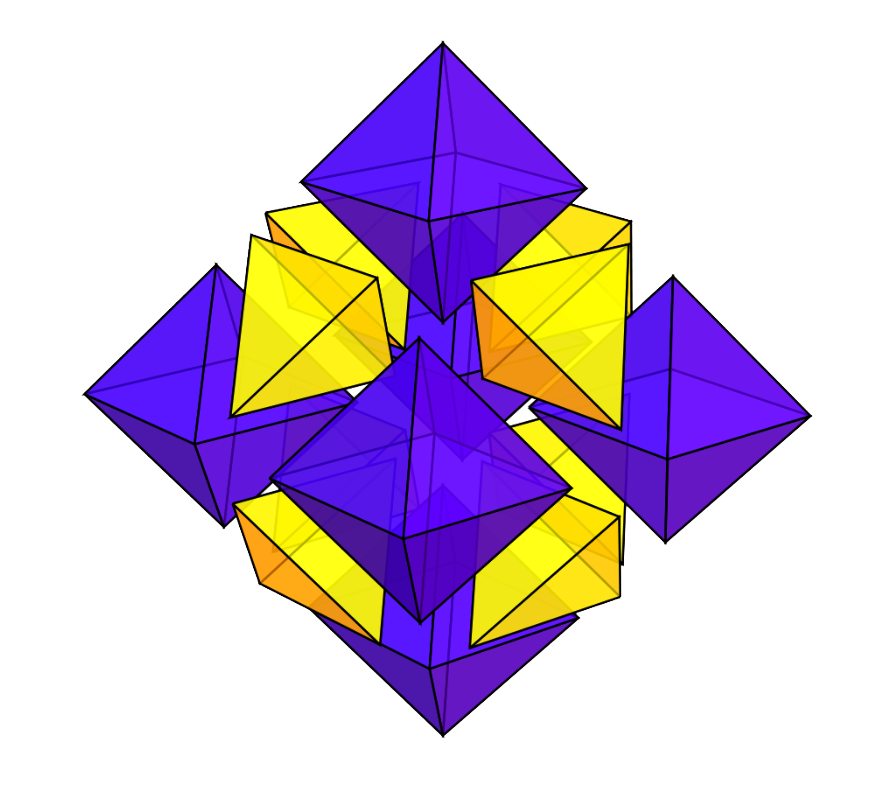
\includegraphics[height = 3cm]{./FigureLayout/tetra-exploded.PNG}
\end{center}


\end{column}%
\end{columns}



\end{frame}




%%%%% =====================================================================================
\begin{frame}\frametitle{Laguerre-Delaunay}
	\framesubtitle{Power distance} 

\begin{itemize}
	\item Generating points are now both locations and \alert{weights}. Can be geometrically interpreted as \alert{spheres}. 
\item $\gamma = \{p_1,\dots, p_n \} = \{(p'_1, p''_1), \dots , (p'_n, p''_n)\}$ can be thought of as \alert{marked point process}.
\item $\gamma \subset \mathbb R^3\times S$, where $S=[0,W], W>0$.
\item Distance is not Euclidean, but the \alert{power distance}
	$$ d(q',p) = \|q'-p'\|^2 - p''.$$
\end{itemize}

\vspace{-4mm}

\definecolor{wrwrwr}{rgb}{0.3803921568627451,0.3803921568627451,0.3803921568627451}
\begin{center}
\resizebox{0.65\textwidth}{!}{
	\begin{tikzpicture}[line cap=round,line join=round,>=triangle 45,x=1cm,y=1cm]
\clip(-34.06221132360224,19.559143724639345) rectangle (-8.217986359569402,34.582776229682544);
\draw [line width=4pt,color=wrwrwr] (-22.818487068133912,26.001637556556815) circle (5.131318559036773cm);
\draw [line width=4pt,color=wrwrwr] (-22.15663388793076,31.090093169232418)-- (-15.018487068133922,30.161637556556805);
\draw [line width=4pt,color=wrwrwr] (-22.818487068133912,26.001637556556815)-- (-22.15663388793076,31.090093169232418);
\draw [line width=4pt,color=wrwrwr] (-22.818487068133912,26.001637556556815)-- (-15.018487068133922,30.161637556556805);
\draw (-23.57696780445743,29.46311574805324) node[anchor=north west] {\Huge$\sqrt{p''}$};
\draw (-19.93284265814484,32.36947322670743) node[anchor=north west] {\Huge$\sqrt{d(q',p)}$};
\draw (-14.567259620629372,30.804511507432096) node[anchor=north west] {\Huge$q'$};
\draw (-23.800533764353904,26.08726975361645) node[anchor=north west] {\Huge$p'$};
\draw (0.009240964620983672,0.35482776953204165) node[anchor=north west] {\Huge$p'$};
\draw (0.009240964620983672,0.35482776953204165) node[anchor=north west] {\Huge$p'$};
\draw (0.009240964620983672,0.35482776953204165) node[anchor=north west] {\Huge$p''$};
\begin{scriptsize}
\draw [fill=wrwrwr] (-22.818487068133912,26.001637556556815) circle (2.5pt);
\draw [fill=wrwrwr] (-15.018487068133922,30.161637556556805) circle (2.5pt);
\draw [fill=wrwrwr] (-22.15663388793076,31.090093169232418) circle (2pt);
\end{scriptsize}
\end{tikzpicture}
}

\end{center}


\end{frame}




%%%%% =====================================================================================
\begin{frame}\frametitle{Laguerre-Delaunay}
	\framesubtitle{Characteristic point, regularity}

	{\footnotesize
	\begin{itemize}
		\item Instead of circumscribed ball, we have the \alert{characteristic point} $p_\eta=(p'_\eta,p''_\eta)$. 
			$$d(p'_\eta,p_i) = p''_\eta,\quad \text{for each } i=1,\dots,4.$$
			\vspace{-2mm}
		\item Instead of the empty sphere property, we have \alert{regularity}
			$$\eta \text{ is regular if there is no other point } q\in \gamma \text{ such that } d(p'_\eta,q)<p''_\eta.$$
	\end{itemize}
}

\vspace{-5mm}


$$\mathcal {LD}_4(\gamma) = \{ \eta \subset \gamma: \mathrm{card}(\eta)=4, \eta \text{ is regular} \}$$

\begin{figure}
    \centering
    \begin{minipage}{0.45\textwidth}
        \centering
		\definecolor{wrwrwr}{rgb}{0.3803921568627451,0.3803921568627451,0.3803921568627451}
	\definecolor{dtsfsf}{rgb}{0.8274509803921568,0.1843137254901961,0.1843137254901961}
	\definecolor{rvwvcq}{rgb}{0.08235294117647059,0.396078431372549,0.7529411764705882}

	\begin{figure}[p]
	\centering
	\resizebox{1\textwidth}{!}{
	\begin{tikzpicture}[line cap=round,line join=round,>=triangle 45,x=1cm,y=1cm]
	\clip(2.3675744046034124,-3.243186132465546) rectangle (14.599454494033491,3.8673877603519258);
	\draw [line width=2pt,color=blue] (7.750406282838338,-0.12641314086610173) circle (1.3444225879561709cm);
	\draw [line width=2pt,color=wrwrwr] (8.501849676455937,1.7651512637575348) circle (1.6272966331795844cm);
	\draw [line width=2pt,color=wrwrwr] (8.890527293844368,-1.111063104916762) circle (0.6436367819392179cm);
	\draw [line width=2pt,color=wrwrwr] (6.480726066036172,-1.2924459930313563) circle (1.0999568941983233cm);
	\draw [color=dtsfsf](7.488880601216007,-0.0476603651576942) node[anchor=north west] {$p_\eta$};
	\begin{scriptsize}
	\draw [fill=rvwvcq] (7.750406282838338,-0.12641314086610173) circle (0.5pt);
	\draw [fill=rvwvcq] (8.501849676455937,1.7651512637575348) circle (0.5pt);
	\draw [fill=rvwvcq] (8.890527293844368,-1.111063104916762) circle (0.5pt);
	\draw [fill=rvwvcq] (6.480726066036172,-1.2924459930313563) circle (0.5pt);
	\end{scriptsize}
	\end{tikzpicture}
	}
	\caption{\scriptsize Points of $\eta$ (gray) and their characteristic point $p_\eta$ (blue).}
\label{fig:Laguerrecospherical}
\end{figure}
    \end{minipage}\hfill
    \begin{minipage}{0.45\textwidth}
        \centering
\begin{figure}[p]
	\centering
	\resizebox{1\textwidth}{!}{
		\definecolor{wrwrwr}{rgb}{0.3803921568627451,0.3803921568627451,0.3803921568627451}
	\definecolor{dtsfsf}{rgb}{0.8274509803921568,0.1843137254901961,0.1843137254901961}
	\definecolor{rvwvcq}{rgb}{0.08235294117647059,0.396078431372549,0.7529411764705882}
\begin{tikzpicture}[line cap=round,line join=round,>=triangle 45,x=1cm,y=1cm]
\clip(2.3675744046034124,-3.243186132465546) rectangle (14.599454494033491,3.8673877603519258);
\draw [line width=2pt,color=blue] (7.750406282838338,-0.12641314086610173) circle (1.3444225879561709cm);
\draw [line width=2pt,color=red] (7,0.5) circle (0.924874885928139cm);
\draw [line width=2pt,color=wrwrwr] (8.501849676455937,1.7651512637575348) circle (1.6272966331795844cm);
\draw [line width=2pt,color=wrwrwr] (8.890527293844368,-1.111063104916762) circle (0.6436367819392179cm);
\draw [line width=2pt,color=wrwrwr] (6.480726066036172,-1.2924459930313563) circle (1.0999568941983233cm);
\draw [color=dtsfsf](7.488880601216007,-0.0476603651576942) node[anchor=north west] {$p_\eta$};
\begin{scriptsize}
\draw [fill=rvwvcq] (7.750406282838338,-0.12641314086610173) circle (0.5pt);
\draw [fill=rvwvcq] (7,0.5) circle (0.5pt);
\draw [fill=rvwvcq] (8.501849676455937,1.7651512637575348) circle (0.5pt);
\draw [fill=rvwvcq] (8.890527293844368,-1.111063104916762) circle (0.5pt);
\draw [fill=rvwvcq] (6.480726066036172,-1.2924459930313563) circle (0.5pt);
\end{scriptsize}
\end{tikzpicture}
}
\caption{\scriptsize A point (red) breaking the regularity of $\eta$.}
\label{fig:Laguerrecospherical}
\end{figure}
    \end{minipage}
\end{figure}

\vspace{-4mm}

\end{frame}





%%%%% =====================================================================================
\begin{frame}\frametitle{Practical results}
	\framesubtitle{Implementation}

	The partition function $Z^z_\Lambda$ is unknown $\rightarrow$ Birth-Death-Move Metropolis-Hastings algorithm. \newline
	Each step has to reconstruct a new tetrahedrization.
	
\begin{center}
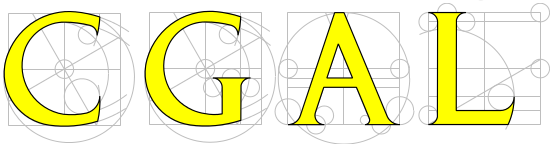
\includegraphics[height = 1cm]{./FigureLayout/cgal.png}
\end{center}


\begin{itemize}
	\item Final solution: implement the MCMC algorithm and rely on Computer Graphics Algorithms Library for handling the tetrahedrization. \newline
		{\footnotesize Current version at \alert{https://github.com/DahnJ/Gibbs-Laguerre-Delaunay.git}}
	\item Simulations done in \texttt{C++}, numerical analysis in \texttt{Python} and \texttt{Mathematica}.
\end{itemize}

\end{frame}



%%%%% =====================================================================================
\begin{frame}\frametitle{Theoretical results}

	{\small

	\alert{\textbf{Goal}}: To prove the existence of the Gibbs-Laguerre-Delaunay models we simulated.
	

	\alert{\textbf{Results}}: Proved the existence of the following two classes of models.

	\vspace{5mm}
	
	A hyperedge potential $\phi$ is \alert{unary} for the hypergraph structure $\mathcal E$ if there exists a measurable function $\hat\varphi:\mathbf N_{lf} \to \mathbb R \cup \{+\infty\}$ such that
	$$\varphi(\eta,\gamma) = \hat\varphi(\eta) \text{ for } \eta \in \mathcal E(\gamma).$$

	\noindent \textbf{Bounded interaction}:  For $\eta\in\mathcal {LD}_4(\gamma)$ define the potential $\varphi_S$ as a unary potential such that
$$\varphi_S(\eta,\gamma) \leq K_0 + K_1 \chi(\eta)^{\beta}$$
for some $K_0,K_1 \geq 0, \beta >0$\newline
	\textbf{Hard-core interaction}: For $\eta\in\mathcal {LD}_4(\gamma)$ define the potential $\varphi_{HC}$ as a unary potential such that
$$\sup_{\eta: d_0 \leq \chi(\eta) \leq d_1} \varphi_{HC}(\eta,\gamma)  < \infty \text{ and } \varphi_{HC}(\eta,\gamma)=\infty \text{ if } \chi(\eta)>\alpha$$ 
for some $0\leq d_0 < d_1 \leq \alpha$. 


	}






\end{frame}



%%%%% Hypergraphs
%%%%% =====================================================================================
\begin{frame}\frametitle{Tessellations as hypergraphs}

Based on \textit{Dereudre, Drouilhet, Georgii: Existence of gibbsian point processes with geometry-dependent interactions (2012)}. \newline



\mffboxTitle{\textbf{Definition}. Hypergraph structure}{
	A \textit{hypergraph structure} is a measurable subset $\mathcal E$ of $(\mathbf N_f\times \mathbf N_{lf}, \mathcal N_f \otimes \mathcal N_{lf})$ such that $\eta \subset \gamma$ for all $(\eta,\gamma)\in\mathcal E$. We call $\eta$ a \textit{hyperedge} of $\gamma$ and write $\eta \in \mathcal E(\gamma)$, where $\mathcal E(\gamma) = \{\eta: (\eta,\gamma) \in \mathcal E\}$. For a given $\gamma \in \mathbf N_{lf}$, the pair $(\gamma, \mathcal E(\gamma))$ is called a \textit{hypergraph}.
}
	\vspace{3mm}
A \alert{hyperedge potential} is a measurable function $\varphi:\mathcal E\to \mathbb R \cup \{+\infty\}$. \newline
We define $\varphi=0$ on $\mathcal E^c$.







\end{frame}






%%%%% =====================================================================================
\begin{frame}\frametitle{Many-body interaction}



	$$ \mathrm{LC}_r = \{(\eta, \gamma) : \eta \subset \gamma, \mathrm{diam}(\eta) \leq r, \gamma \in \mathbb N_{lf} \}$$


\definecolor{ffqqtt}{rgb}{1,0,0.2}
\definecolor{qqzzff}{rgb}{0,0.6,1}
\definecolor{wrwrwr}{rgb}{0.3803921568627451,0.3803921568627451,0.3803921568627451}
\definecolor{wqwqwq}{rgb}{0.3764705882352941,0.3764705882352941,0.3764705882352941}
\definecolor{rvwvcq}{rgb}{0.08235294117647059,0.396078431372549,0.7529411764705882}

\begin{tikzpicture}[line cap=round,line join=round,>=triangle 45,x=1cm,y=1cm]
\draw [line width=1pt,dash pattern=on 1pt off 1pt,color=wqwqwq] (-5.651363174596976,3.076327618564131) circle (1cm);
\draw [line width=1pt,dash pattern=on 1pt off 1pt,color=wqwqwq] (-4.064010038277704,1.9432780672854815) circle (1cm);
\draw [line width=1pt,dash pattern=on 1pt off 1pt,color=wqwqwq] (-5.571363174596976,2.3363276185641313) circle (1cm);
\draw [line width=1pt,dash pattern=on 1pt off 1pt,color=wqwqwq] (-5.031363174596976,2.696327618564131) circle (1cm);
\draw [line width=1pt,dash pattern=on 1pt off 1pt,color=wqwqwq] (-4.26712854600867,2.49918135160181) circle (1cm);
\draw [line width=1pt,dash pattern=on 1pt off 1pt,color=wqwqwq] (-3.78605839611954,2.4029673216239837) circle (1cm);
\draw [line width=1pt,dash pattern=on 1pt off 1pt,color=wqwqwq] (-3.2408455595785255,2.9267992626143706) circle (1cm);
\draw [line width=1pt,color=wrwrwr] (0.6067459162602004,4.07133190226534)-- (1.3709805448485053,3.874185635303018);
\draw [line width=1pt,color=wrwrwr] (1.3709805448485053,3.874185635303018)-- (1.5740990525794705,3.3182823509866894);
\draw [line width=1pt,color=wrwrwr] (1.5740990525794705,3.3182823509866894)-- (1.8520506947376343,3.777971605325192);
\draw [line width=1pt,color=wrwrwr] (1.8520506947376343,3.777971605325192)-- (1.3709805448485053,3.874185635303018);
\draw [line width=1pt,color=wrwrwr] (1.8520506947376343,3.777971605325192)-- (2.3972635312786474,4.30180354631558);
\draw [line width=1pt,color=wrwrwr] (-0.013254083739799749,4.45133190226534)-- (0.6067459162602004,4.07133190226534);
\draw [line width=1pt,color=wrwrwr] (0.06674591626020032,3.7113319022653393)-- (0.6067459162602004,4.07133190226534);
\draw [line width=1pt,color=wrwrwr] (0.06674591626020032,3.7113319022653393)-- (-0.013254083739799749,4.45133190226534);
\draw [line width=1pt,color=wrwrwr] (0.5596237030915541,0.6537664662158094)-- (1.3238583316798593,0.45662019925348796);
\draw [line width=1pt,color=wrwrwr] (1.3238583316798593,0.45662019925348796)-- (1.526976839410824,-0.09928308506284056);
\draw [line width=1pt,color=wrwrwr] (1.526976839410824,-0.09928308506284056)-- (1.8049284815689877,0.36040616927566216);
\draw [line width=1pt,color=wrwrwr] (1.8049284815689877,0.36040616927566216)-- (1.3238583316798593,0.45662019925348796);
\draw [line width=1pt,color=wrwrwr] (1.8049284815689877,0.36040616927566216)-- (2.3501413181100013,0.8842381102660499);
\draw [line width=1pt,color=wrwrwr] (-0.06037629690844604,1.0337664662158104)-- (0.5596237030915541,0.6537664662158094);
\draw [line width=1pt,color=wrwrwr] (0.019623703091554034,0.29376646621580926)-- (0.5596237030915541,0.6537664662158094);
\draw [line width=1pt,color=wrwrwr] (0.019623703091554034,0.29376646621580926)-- (-0.06037629690844604,1.0337664662158104);
\draw [rotate around={-66.05441581138116:(0.21510616832432855,0.640401043804194)},line width=1pt,color=qqzzff,fill=qqzzff,fill opacity=0.22] (0.21510616832432855,0.640401043804194) ellipse (0.5892588021493973cm and 0.44624664441269635cm);
\draw [rotate around={-73.7478395632461:(1.5555433584785359,0.21708092057793912)},line width=1pt,color=ffqqtt,fill=ffqqtt,fill opacity=0.2] (1.5555433584785359,0.21708092057793912) ellipse (0.5262034058004502cm and 0.342998584347721cm);
\draw [->,line width=1pt,color=wrwrwr] (-1.586430394404893,3.331166353524088) -- (-0.8250976964074973,3.615245718448489);
\draw [->,line width=1pt,color=wrwrwr] (-1.6773357911807014,2.069853973259747) -- (-0.9273662677802819,1.6380533385746578);
\begin{scriptsize}
\draw [fill=rvwvcq] (-5.651363174596976,3.076327618564131) circle (2.5pt);
\draw [fill=rvwvcq] (-4.064010038277704,1.9432780672854815) circle (2.5pt);
\draw [fill=rvwvcq] (-5.571363174596976,2.3363276185641313) circle (2.5pt);
\draw [fill=rvwvcq] (-5.031363174596976,2.696327618564131) circle (2.5pt);
\draw [fill=rvwvcq] (-4.26712854600867,2.49918135160181) circle (2.5pt);
\draw [fill=rvwvcq] (-3.78605839611954,2.4029673216239837) circle (2.5pt);
\draw [fill=rvwvcq] (-3.2408455595785255,2.9267992626143706) circle (2.5pt);
\draw [fill=rvwvcq] (-0.013254083739799749,4.45133190226534) circle (2.5pt);
\draw [fill=rvwvcq] (1.5740990525794705,3.3182823509866894) circle (2.5pt);
\draw [fill=rvwvcq] (0.06674591626020032,3.7113319022653393) circle (2.5pt);
\draw [fill=rvwvcq] (0.6067459162602004,4.07133190226534) circle (2.5pt);
\draw [fill=rvwvcq] (1.3709805448485053,3.874185635303018) circle (2.5pt);
\draw [fill=rvwvcq] (1.8520506947376343,3.777971605325192) circle (2.5pt);
\draw [fill=rvwvcq] (2.3972635312786474,4.30180354631558) circle (2.5pt);
\draw [fill=rvwvcq] (-0.06037629690844604,1.0337664662158104) circle (2.5pt);
\draw [fill=rvwvcq] (1.526976839410824,-0.09928308506284056) circle (2.5pt);
\draw [fill=rvwvcq] (0.019623703091554034,0.29376646621580926) circle (2.5pt);
\draw [fill=rvwvcq] (0.5596237030915541,0.6537664662158094) circle (2.5pt);
\draw [fill=rvwvcq] (1.3238583316798593,0.45662019925348796) circle (2.5pt);
\draw [fill=rvwvcq] (1.8049284815689877,0.36040616927566216) circle (2.5pt);
\draw [fill=rvwvcq] (2.3501413181100013,0.8842381102660499) circle (2.5pt);
\end{scriptsize}
\end{tikzpicture}

\end{frame}



%%%%% =====================================================================================
\begin{frame}[noframenumbering]\frametitle{Set $\mathcal E_\Lambda$}

% $$\mathbf N_\Lambda = \{ \nu \in \mathbf N_{lf}: \nu( (\mathbb R^3 \setminus \Lambda) \times S) = 0 \}$$

Let $\Lambda \in \mathcal B_0$. Define the set 
	$$\mathcal E_\Lambda(\gamma) := \{ \eta \in \mathcal E(\gamma): \varphi(\eta,\zeta \cup \gamma_{\Lambda^c}) \neq \varphi(\eta,\gamma) \text{ for some } \zeta \in \mathbf N_\Lambda \}.$$


For $\eta \in \mathcal E(\gamma)$ such that $\varphi(\eta,\gamma)\neq 0$ we have the following implication:
$$\eta \notin \mathcal E(\zeta \cup \gamma_{\Lambda^c})\text{ for some }\zeta \in \mathbf N_{\Lambda} \Rightarrow \eta \in \mathcal E_{\Lambda}(\gamma).$$ 

\definecolor{xdxdff}{rgb}{0.49019607843137253,0.49019607843137253,1}
\definecolor{rvwvcq}{rgb}{0.08235294117647059,0.396078431372549,0.7529411764705882}
\definecolor{ffzzcc}{rgb}{1,0.6,0.8}
\definecolor{ffqqtt}{rgb}{1,0,0.2}
\definecolor{ffttww}{rgb}{1,0.2,0.4}
	\begin{center}
\resizebox{0.3\textwidth}{!}{
\begin{tikzpicture}[line cap=round,line join=round,>=triangle 45,x=1cm,y=1cm]
\fill[line width=0.5pt,color=ffttww,fill=ffttww,fill opacity=0.10000000149011612] (0,0) -- (1,0) -- (1,1) -- (0,1) -- cycle;
\fill[line width=0.5pt,color=ffqqtt,fill=ffqqtt,fill opacity=0.10000000149011612] (-0.6340997915074242,1.3877207078549374) -- (-0.5774919676583712,0.8640983372511976) -- (-0.3416260349539835,1.57169613536436) -- cycle;
\fill[line width=0.5pt,color=rvwvcq,fill=rvwvcq,fill opacity=0.10000000149011612] (-0.5161668251552307,0.09989271528898214) -- (-0.11991205821185927,0.3357586479933692) -- (-0.06802155301689386,0.04328489143992931) -- cycle;
\draw [line width=0.5pt,color=ffttww] (0,0)-- (1,0);
\draw [line width=0.5pt,color=ffttww] (1,0)-- (1,1);
\draw [line width=0.5pt,color=ffttww] (1,1)-- (0,1);
\draw [line width=0.5pt,color=ffttww] (0,1)-- (0,0);
\draw [line width=0.5pt,color=ffqqtt] (-0.6340997915074242,1.3877207078549374)-- (-0.5774919676583712,0.8640983372511976);
\draw [line width=0.5pt,color=ffqqtt] (-0.5774919676583712,0.8640983372511976)-- (-0.3416260349539835,1.57169613536436);
\draw [line width=0.5pt,color=ffqqtt] (-0.3416260349539835,1.57169613536436)-- (-0.6340997915074242,1.3877207078549374);
\draw [line width=0.5pt,color=ffzzcc] (-0.28699178319490615,1.1603748302706884) circle (0.414933871224362cm);
\draw [line width=0.5pt,color=rvwvcq] (-0.5161668251552307,0.09989271528898214)-- (-0.11991205821185927,0.3357586479933692);
\draw [line width=0.5pt,color=rvwvcq] (-0.11991205821185927,0.3357586479933692)-- (-0.06802155301689386,0.04328489143992931);
\draw [line width=0.5pt,color=rvwvcq] (-0.06802155301689386,0.04328489143992931)-- (-0.5161668251552307,0.09989271528898214);
\draw [line width=0.5pt,color=xdxdff] (-0.2813978861427192,0.15626786833258824) circle (0.24144277294164407cm);
\end{tikzpicture}
}
	\end{center}


Finite horizon, range confinement, range condition.

\end{frame}


%%%%% Pseudo-periodic configurations
%%%%% =====================================================================================
\begin{frame}\frametitle{Pseudo-periodic configurations}

$M\in\mathbb R^{3\times 3}$ $\dots$ an invertible $3\times 3$ matrix, column vectors $(M_1,M_2,M_3)$. \newline
	For each $k \in \mathbb Z^3$ define the cell
$$C(k) =  \{Mx \in \mathbb R^3: x-k \in \left[ -1/2, 1/2 \right)^3 \}.$$
Let $\Gamma \in \mathcal N_C$ be non-empty. Then we define the \textit{pseudo-periodic} configurations $\bar \Gamma$ as
$$\bar \Gamma = \{ \gamma \in \mathbf N_{lf}: \vartheta_{Mk}(\gamma_{C(k)}) \in \Gamma \text{ for all } k \in \mathbb Z^3 \},$$

\noindent Fix some $A \subset C\times S$ and define
	$$\Gamma^b = \{\zeta \in \mathbf N_C: \zeta = \{p\}, p \in B(0,b)\},$$

Let $M$ be such that $|M_i| = a > 0$ for $i=1,2,3$ and $\angle(M_i,M_j) = \pi / 3$ for $i\neq j$.




\end{frame}






%%%%% =====================================================================================
\begin{frame}


	\center\large\alert{In 2D: Equilateral triangles }

\definecolor{aqaqaq}{rgb}{0.6274509803921569,0.6274509803921569,0.6274509803921569}

\definecolor{wrwrwr}{rgb}{0.3803921568627451,0.3803921568627451,0.3803921568627451}
\begin{center}

\resizebox{0.6\textwidth}{!}{
\begin{tikzpicture}[line cap=round,line join=round,>=triangle 45,x=1cm,y=1cm]
\draw [line width=0.8pt,color=aqaqaq] (0,4)-- (0,0);
\draw [line width=0.8pt,color=aqaqaq] (0.8660254037844386,3.5)-- (0.8660254037844386,0.5);
\draw [line width=0.8pt,color=aqaqaq] (1.7320508075688772,4)-- (1.7320508075688772,0);
\draw [line width=0.8pt,color=aqaqaq] (2.598076211353316,3.5)-- (2.598076211353316,0.5);
\draw [line width=0.8pt,color=aqaqaq] (3.4641016151377544,4)-- (3.4641016151377544,0);
\draw [line width=0.8pt,color=aqaqaq] (0,2)-- (3.4641016151377544,0);
\draw [line width=0.8pt,color=aqaqaq] (0,1)-- (1.7320508075688772,0);
\draw [line width=0.8pt,color=aqaqaq] (0,2)-- (3.4641016151377544,4);
\draw [line width=0.8pt,color=aqaqaq] (0,3)-- (1.7320508075688772,4);
\draw [line width=0.8pt,color=aqaqaq] (0,1)-- (5.196152422706632,4);
\draw [line width=0.8pt,color=aqaqaq] (0,0)-- (5.196152422706632,3);
\draw [line width=0.8pt,color=aqaqaq] (1.7320508075688772,0)-- (5.196152422706632,2);
\draw [line width=0.8pt,color=aqaqaq] (3.4641016151377544,4)-- (5.196152422706632,3);
\draw [line width=0.8pt,color=aqaqaq] (1.7320508075688772,4)-- (5.196152422706632,2);
\draw [line width=0.8pt,color=aqaqaq] (0,4)-- (5.196152422706632,1);
\draw [line width=0.8pt,color=aqaqaq] (0,3)-- (5.196152422706632,0);
\draw [line width=0.8pt,color=aqaqaq] (3.4641016151377544,0)-- (5.196152422706632,1);
\draw [line width=0.8pt,color=aqaqaq] (4.330127018922193,3.5)-- (4.330127018922193,0.5);
\draw [line width=0.8pt,color=aqaqaq] (5.196152422706632,4)-- (5.196152422706632,0);
\begin{scriptsize}
\draw [fill=aqaqaq] (0,0) circle (1.5pt);
\draw [fill=aqaqaq] (0,1) circle (1.5pt);
\draw [fill=aqaqaq] (0.8660254037844386,0.5) circle (1.5pt);
\draw [fill=aqaqaq] (0,2) circle (1.5pt);
\draw [fill=aqaqaq] (0,3) circle (1.5pt);
\draw [fill=aqaqaq] (0,4) circle (1.5pt);
\draw [fill=aqaqaq] (0.8660254037844386,1.5) circle (1.5pt);
\draw [fill=aqaqaq] (0.8660254037844386,2.5) circle (1.5pt);
\draw [fill=aqaqaq] (0.8660254037844386,3.5) circle (1.5pt);
\draw [fill=aqaqaq] (1.7320508075688772,4) circle (1.5pt);
\draw [fill=aqaqaq] (1.7320508075688772,3) circle (1.5pt);
\draw [fill=aqaqaq] (1.7320508075688772,2) circle (1.5pt);
\draw [fill=aqaqaq] (1.7320508075688772,1) circle (1.5pt);
\draw [fill=aqaqaq] (1.7320508075688772,0) circle (1.5pt);
\draw [fill=aqaqaq] (2.598076211353316,3.5) circle (1.5pt);
\draw [fill=aqaqaq] (2.598076211353316,2.5) circle (1.5pt);
\draw [fill=aqaqaq] (2.598076211353316,1.5) circle (1.5pt);
\draw [fill=aqaqaq] (2.598076211353316,0.5) circle (1.5pt);
\draw [fill=aqaqaq] (3.4641016151377544,4) circle (1.5pt);
\draw [fill=aqaqaq] (3.4641016151377544,3) circle (1.5pt);
\draw [fill=aqaqaq] (3.4641016151377544,2) circle (1.5pt);
\draw [fill=aqaqaq] (3.4641016151377544,1) circle (1.5pt);
\draw [fill=aqaqaq] (3.4641016151377544,0) circle (1.5pt);
\draw [fill=aqaqaq] (4.330127018922193,3.5) circle (1.5pt);
\draw [fill=aqaqaq] (4.330127018922193,2.5) circle (1.5pt);
\draw [fill=aqaqaq] (4.330127018922193,1.5) circle (1.5pt);
\draw [fill=aqaqaq] (4.330127018922193,0.5) circle (1.5pt);
\draw [fill=aqaqaq] (5.196152422706632,4) circle (1.5pt);
\draw [fill=aqaqaq] (5.196152422706632,3) circle (1.5pt);
\draw [fill=aqaqaq] (5.196152422706632,2) circle (1.5pt);
\draw [fill=aqaqaq] (5.196152422706632,1) circle (1.5pt);
\draw [fill=aqaqaq] (5.196152422706632,0) circle (1.5pt);
\end{scriptsize}
\end{tikzpicture}
}

\end{center}
\end{frame}



%%%%% =====================================================================================
\begin{frame}[plain]



	\only<1-2> {	\center\large\alert{In 3D: Regular tetrahedra?}
	    \only<2>{\begin{figure}
	\begin{center}
		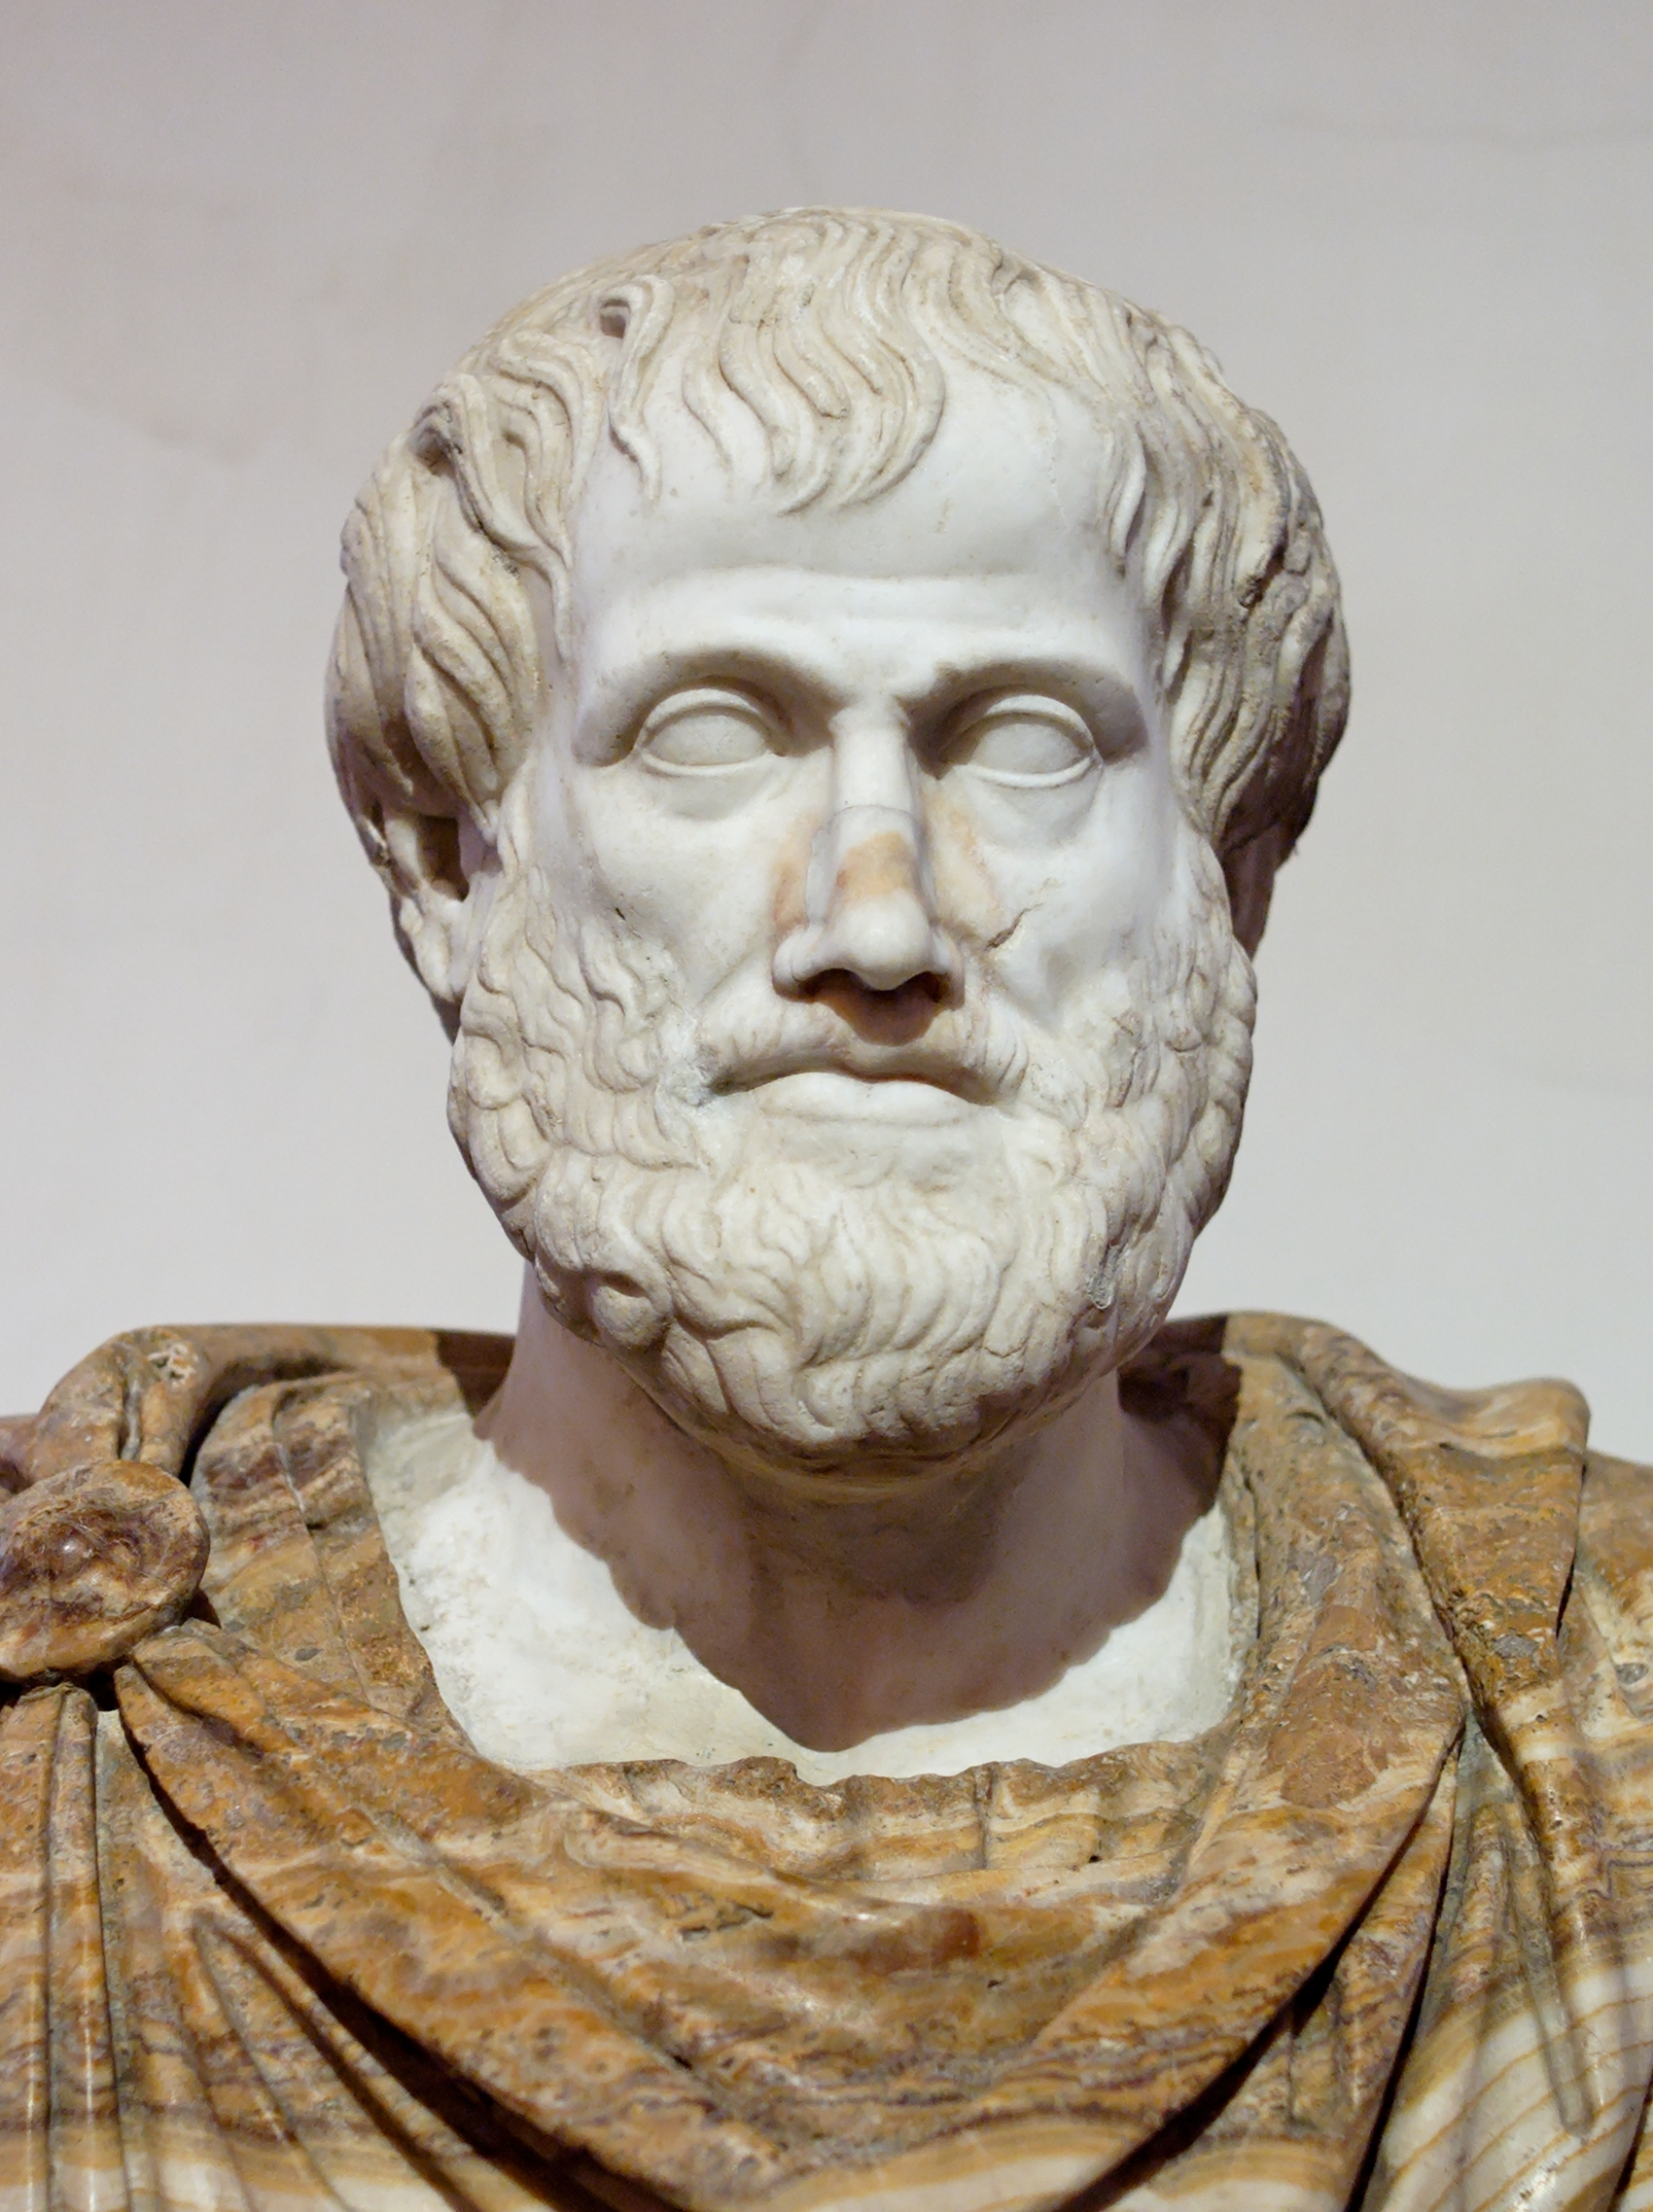
\includegraphics[height = 5cm]{./FigureLayout/aristotle.jpg}
	\end{center}
	\caption{\scriptsize Aristotle}
\end{figure}
	}
}
	\only<3>{ \center\large\alert{In 3D: \sout{Regular tetrahedra}}

	\begin{figure}
	\begin{center}
		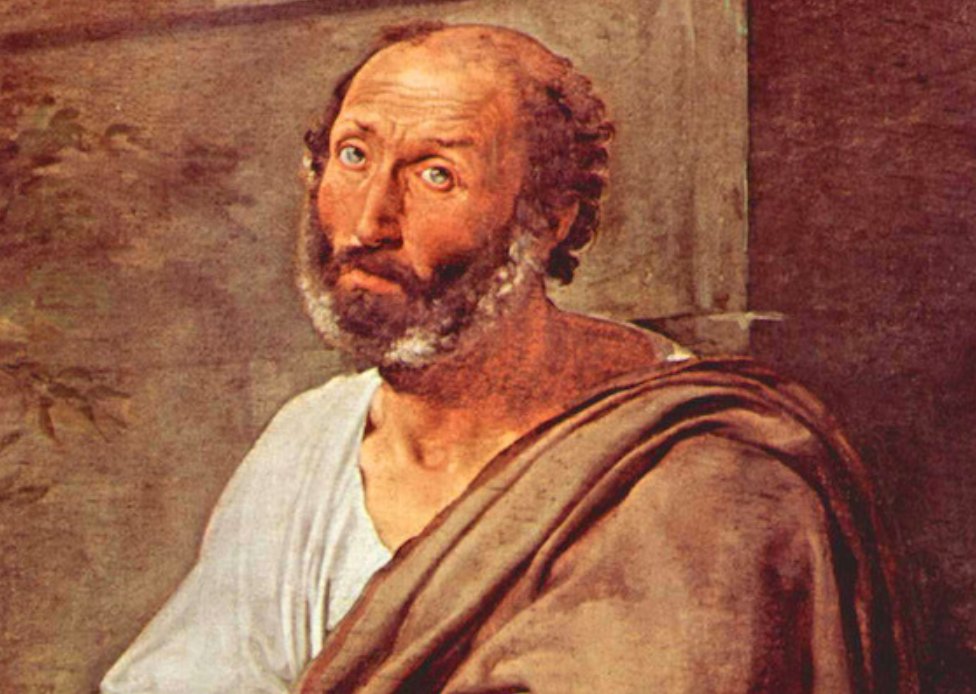
\includegraphics[height = 5cm]{./FigureLayout/aristotlesad.PNG}
	\end{center}
	\caption{\scriptsize Tetrahedrons do not tessellate.}
\end{figure}

	
	
	
	}



	\only<4> {	\center\large\alert{In 3D: Tetrahedral-octahedral honeycomb}

\begin{figure}
    \centering
    \begin{minipage}{0.45\textwidth}
	    \begin{figure}
	\begin{center}
		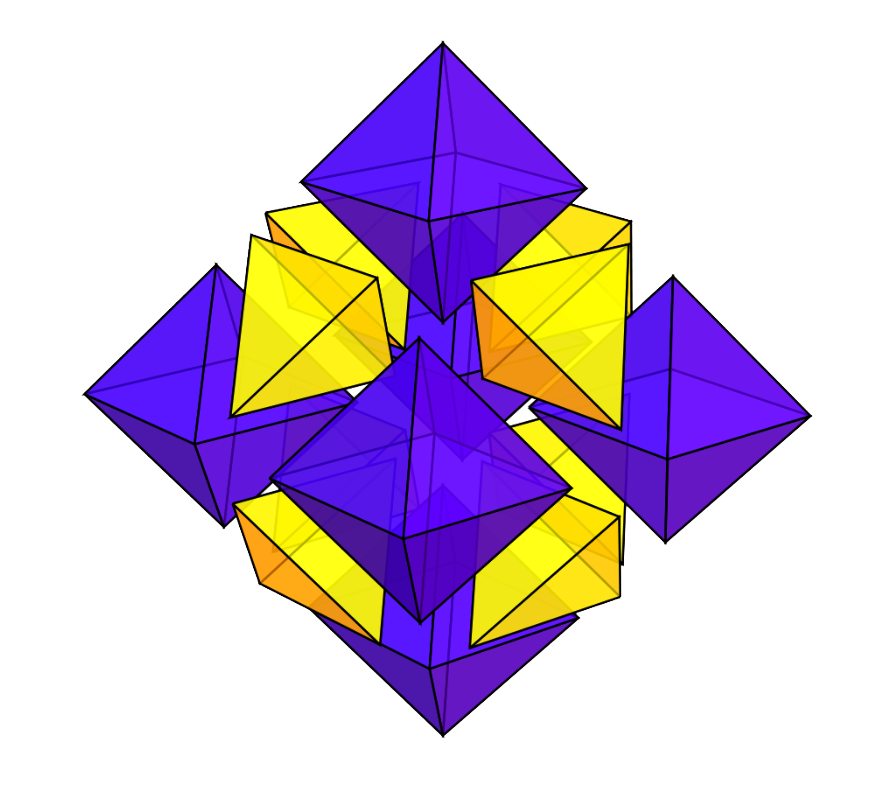
\includegraphics[height = 3cm]{./FigureLayout/tetra-exploded.PNG}
	\end{center}
	\caption{\scriptsize Tetrahedral-octahedral honeycomb in an exploded view.}
\end{figure}
    \end{minipage}\hfill
    \begin{minipage}{0.45\textwidth}
        \centering
\begin{figure}[p]

	\begin{center}
		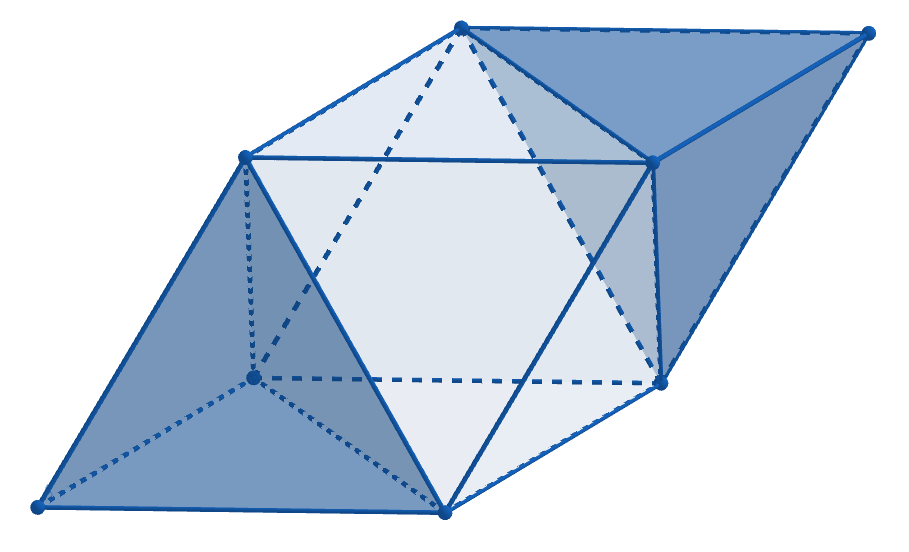
\includegraphics[height = 3cm]{./FigureLayout/tetra-tess.png}
	\end{center}

	\caption{\scriptsize A single cell of a tetrahedral-octahedral honeycomb.}
\end{figure}
    \end{minipage}
\end{figure}
}



\end{frame}



%%%%% =====================================================================================
\begin{frame}[plain]
	% \frametitle{Octet truss}


	\begin{center}
		\only<1>{	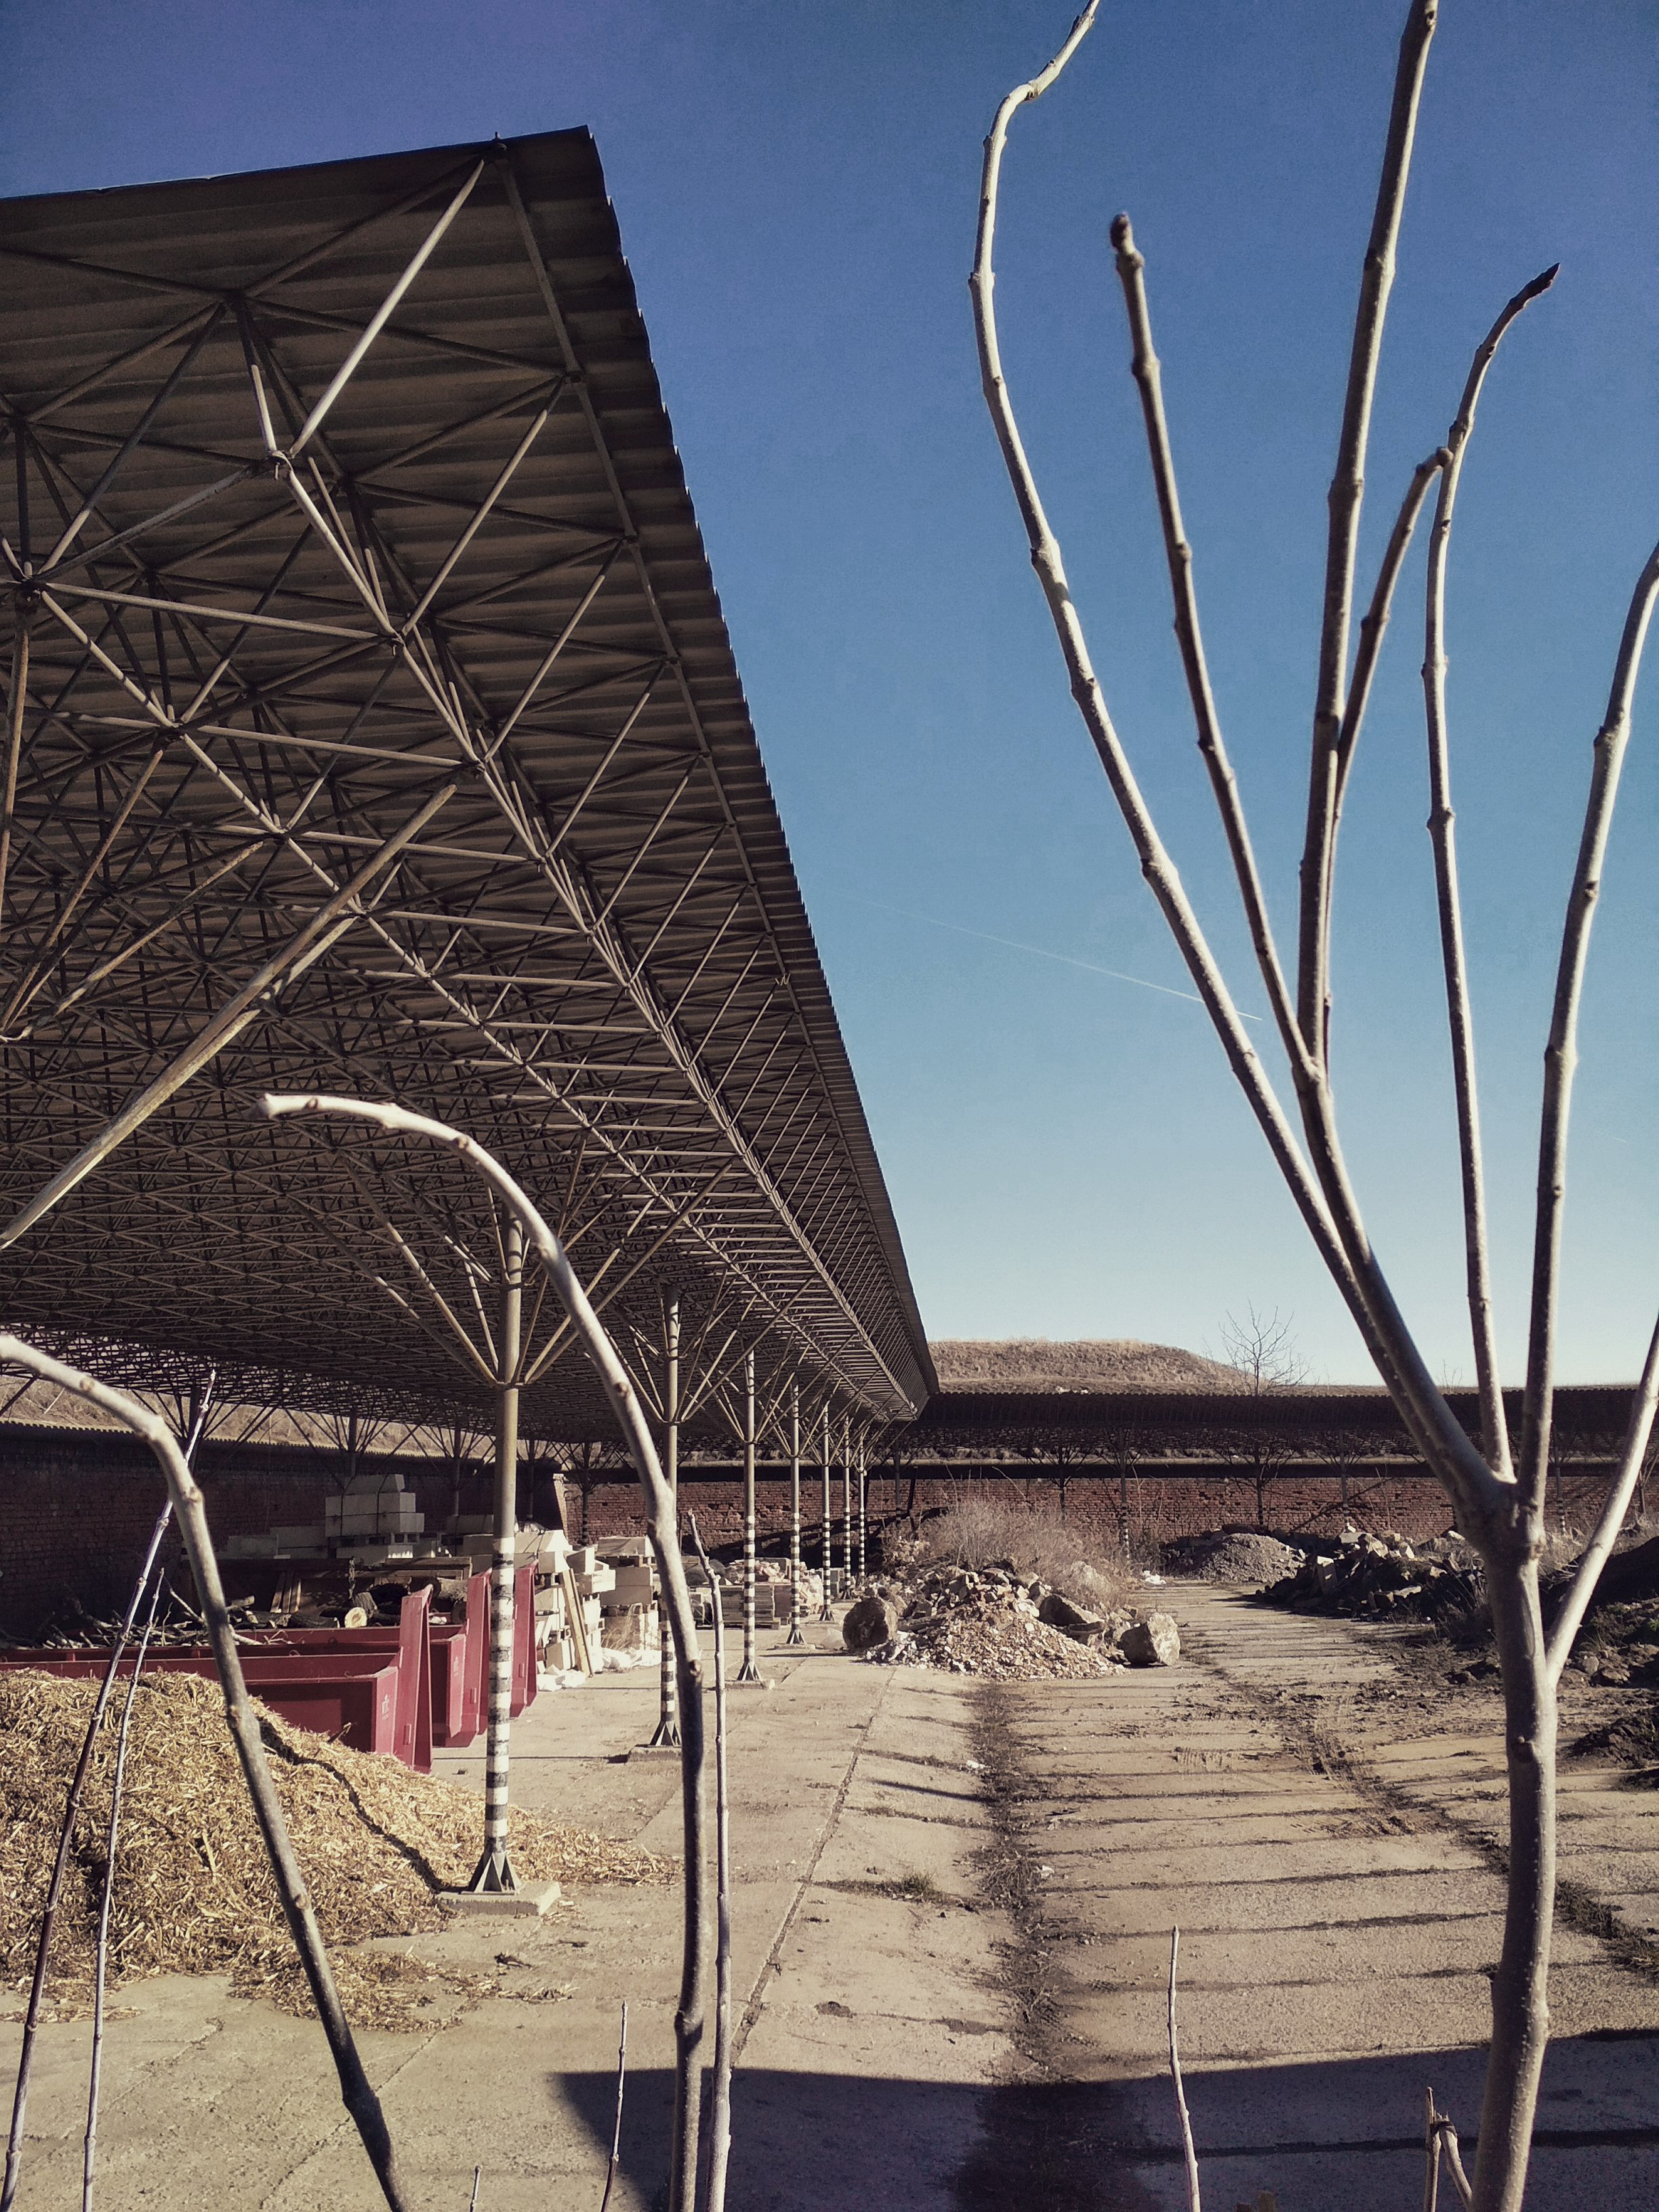
\includegraphics[height = 8cm]{./FigureLayout/terezin2.jpg}}
		\only<2>{	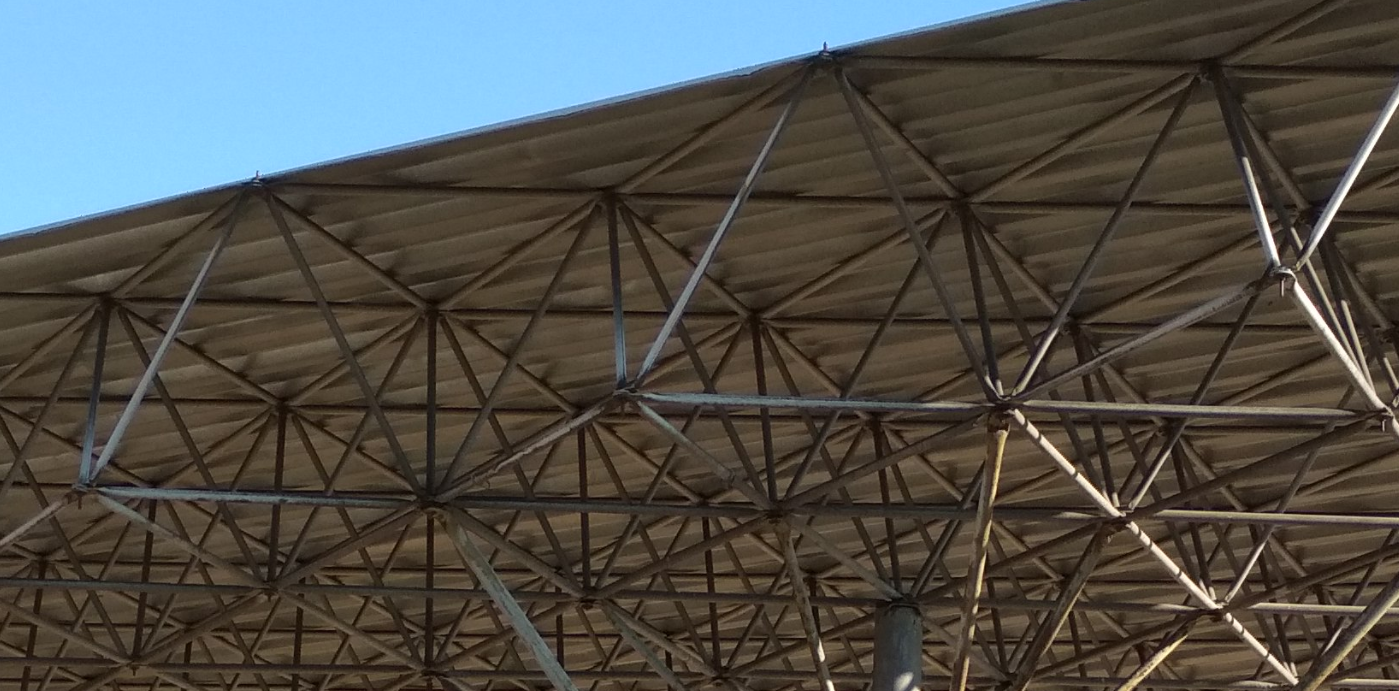
\includegraphics[height = 5cm]{./FigureLayout/truss.PNG}}
		\only<3>{	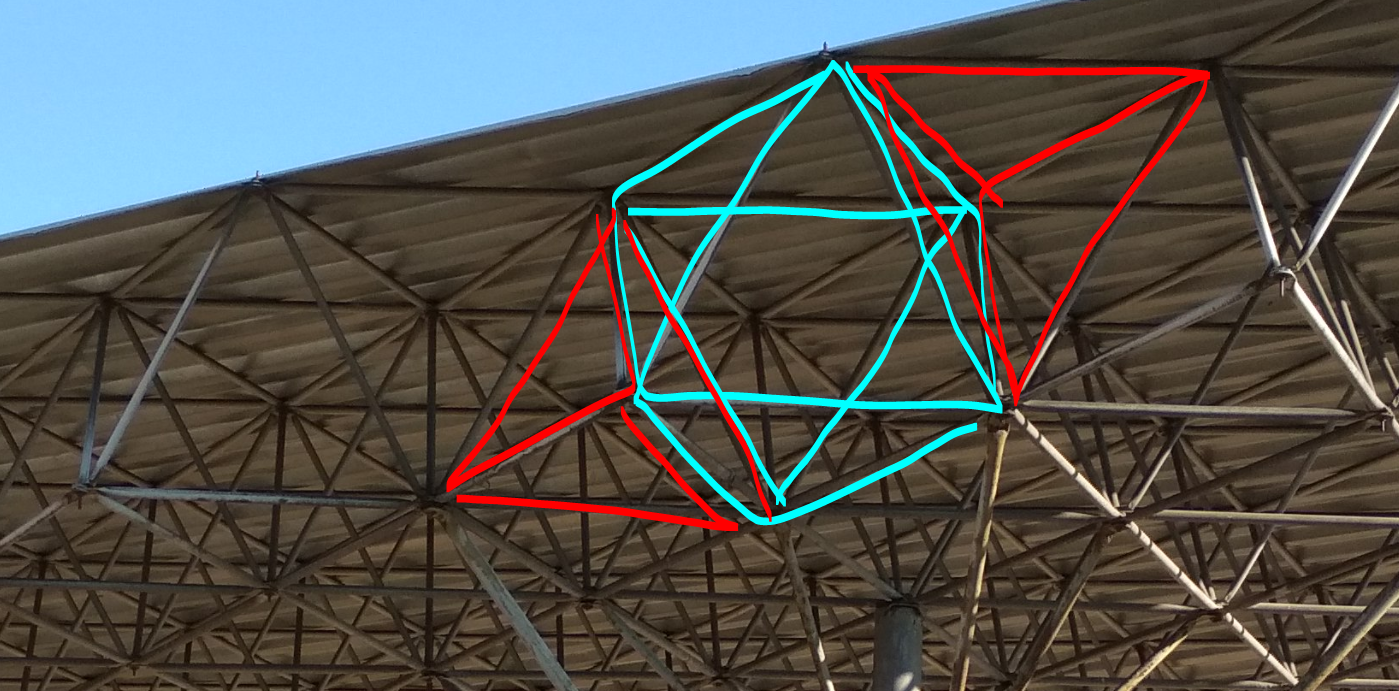
\includegraphics[height = 5cm]{./FigureLayout/truss2.PNG}}
	\end{center}


\end{frame}





%%%%% =====================================================================================
\begin{frame}[plain]


	\begin{center}
			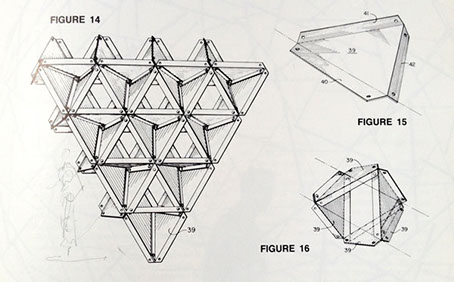
\includegraphics[height = 4cm]{./FigureLayout/truss.jpg}
			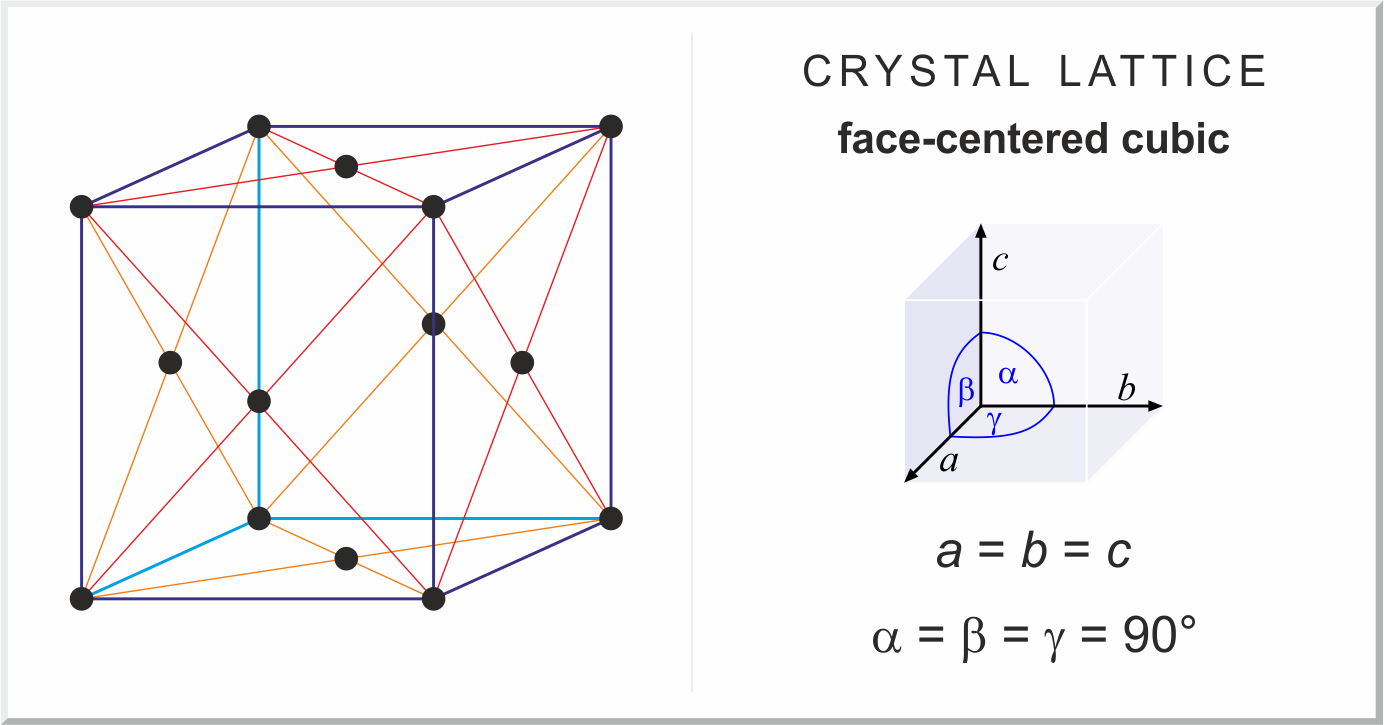
\includegraphics[height = 4cm]{./FigureLayout/fcc.png}
	\end{center}


\end{frame}



%%%%% Bounding the diameter
%%%%% =====================================================================================
\begin{frame}\frametitle{Bounding the diameter}

$$\varphi_S(\eta,\gamma) \leq K_0 + K_1 \chi(\eta)^{\beta}$$
Need to bound the potential on the pseudo-periodic configurations $\tilde \Gamma$.

\definecolor{wrwrwr}{rgb}{0.3803921568627451,0.3803921568627451,0.3803921568627451}
\definecolor{qqwwzz}{rgb}{0,0.4,0.6}
\definecolor{rvwvcq}{rgb}{0.08235294117647059,0.396078431372549,0.7529411764705882}

	\begin{center}
\begin{tikzpicture}[line cap=round,line join=round,>=triangle 45,x=1cm,y=1cm, scale = 3]
\draw [line width=0.3pt,color=qqwwzz,fill=qqwwzz,fill opacity=0.07] (0,0) circle (0.3cm);
\draw [line width=0.3pt,color=qqwwzz,fill=qqwwzz,fill opacity=0.06] (1,0) circle (0.3cm);
\draw [line width=0.3pt,color=qqwwzz,fill=qqwwzz,fill opacity=0.06] (0.5,0.8660254037844386) circle (0.3cm);
\draw [line width=0.3pt,color=rvwvcq] (0,0)-- (1,0);
\draw [line width=0.3pt,color=rvwvcq] (1,0)-- (0.5,0.8660254037844386);
\draw [line width=0.3pt,color=rvwvcq] (0.5,0.8660254037844386)-- (0,0);
\draw [line width=0.4pt,dotted,color=wrwrwr] (0.5,0.2886751345948128) circle (0.5773502691896257cm);
\begin{scriptsize}
\draw [fill=rvwvcq] (0,0) circle (0.5pt);
\draw[color=rvwvcq] (0.020731175192614887,0.053989196036012065) node {$A$};
\draw [fill=rvwvcq] (1,0) circle (0.5pt);
\draw[color=rvwvcq] (1.0202784465226986,0.053989196036012065) node {$B$};
\draw [fill=rvwvcq] (0.5,0.8660254037844386) circle (0.5pt);
\draw[color=rvwvcq] (0.5192768658068827,0.918462511780949) node {$C$};
\end{scriptsize}
\end{tikzpicture}
	\end{center}

\end{frame}



%%%%% =====================================================================================
\begin{frame}[noframenumbering]\frametitle{Problem of Apollonius}




		\begin{center}
\definecolor{ffqqtt}{rgb}{1,0,0.2}
\definecolor{qqwwzz}{rgb}{0,0.4,0.6}
\definecolor{rvwvcq}{rgb}{0.08235294117647059,0.396078431372549,0.7529411764705882}
\begin{tikzpicture}[line cap=round,line join=round,>=triangle 45,x=1cm,y=1cm, scale = 3]
\draw [line width=0.3pt,color=qqwwzz,fill=qqwwzz,fill opacity=0.07] (0,0) circle (0.3cm);
\draw [line width=0.3pt,color=qqwwzz,fill=qqwwzz,fill opacity=0.06] (1,0) circle (0.3cm);
\draw [line width=0.3pt,color=qqwwzz,fill=qqwwzz,fill opacity=0.06] (0.5,0.8660254037844386) circle (0.3cm);
\draw [line width=0.3pt,color=rvwvcq] (0,0)-- (1,0);
\draw [line width=0.3pt,color=rvwvcq] (1,0)-- (0.5,0.8660254037844386);
\draw [line width=0.3pt,color=rvwvcq] (0.5,0.8660254037844386)-- (0,0);
\draw [line width=0.4pt,dash pattern=on 1pt off 1pt,color=orange] (0.4993733260025002,-0.3661748684203649) circle (0.9256483931469245cm);
\draw [line width=0.4pt,dash pattern=on 1pt off 1pt,color=ffqqtt] (0.5,0.28867513459481287) circle (0.27877050834391687cm);
\draw [line width=0.4pt,dash pattern=on 1pt off 1pt,color=blue] (0.5,0.28867513459481287) circle (0.8793764157193666cm);
\begin{scriptsize}
\draw [fill=rvwvcq] (0,0) circle (0.5pt);
\draw[color=rvwvcq] (0.020731175192614887,0.053989196036012065) node {$A$};
\draw [fill=rvwvcq] (1,0) circle (0.5pt);
\draw[color=rvwvcq] (1.0202784465226986,0.053989196036012065) node {$B$};
\draw [fill=rvwvcq] (0.5,0.8660254037844386) circle (0.5pt);
\draw[color=rvwvcq] (0.5192768658068827,0.918462511780949) node {$C$};
\end{scriptsize}
\end{tikzpicture}
\end{center}


% 	\begin{center}
% 		\resizebox{0.7\textwidth}{!}{
% \definecolor{rvwvcq}{rgb}{0.08235294117647059,0.396078431372549,0.7529411764705882}
% \definecolor{wrwrwr}{rgb}{0.3803921568627451,0.3803921568627451,0.3803921568627451}
% \begin{tikzpicture}[line cap=round,line join=round,>=triangle 45,x=1cm,y=1cm]
% \draw [line width=2pt] (-3.539652591272559,2.2876337692195516) circle (3cm);
% \draw [line width=2pt] (2.2825268334159348,5) circle (2.2cm);
% \draw [line width=2pt] (2.6801390868092954,-0.012837125413438684) circle (1cm);
% \draw [line width=2pt,dotted,color=rvwvcq] (0.8641765349861721,1.634714059416633) circle (1.4519675561187415cm);
% \draw [line width=2pt,dotted,color=rvwvcq] (-0.8820533137621848,3.2375500255636234) circle (5.822264129008905cm);
% \begin{scriptsize}
% \draw [fill=wrwrwr] (-3.539652591272559,2.2876337692195516) circle (2.5pt);
% \draw [fill=wrwrwr] (2.2825268334159348,5) circle (2.5pt);
% \draw [fill=wrwrwr] (2.6801390868092954,-0.012837125413438684) circle (2.5pt);
% \draw [fill=wrwrwr] (-6.364617749771356,1.2778952618485286) circle (2.5pt);
% \draw [fill=wrwrwr] (3.41883616048112,-0.6868746861982129) circle (2.5pt);
% \draw [fill=wrwrwr] (1.4280913521046619,2.9727013026501585) circle (2.5pt);
% \draw [fill=wrwrwr] (-0.5720911227217711,1.847657712629322) circle (2.5pt);
% \draw [fill=wrwrwr] (1.9395246576780865,0.6590931294215832) circle (2.5pt);
% \draw [fill=wrwrwr] (4.204550207701663,6.07043269227882) circle (2.5pt);
% \end{scriptsize}
% \end{tikzpicture}
% }
% \end{center}

\end{frame}





%%%%% =====================================================================================
\begin{frame}\frametitle{Apollonius spheres}



\begin{center}
	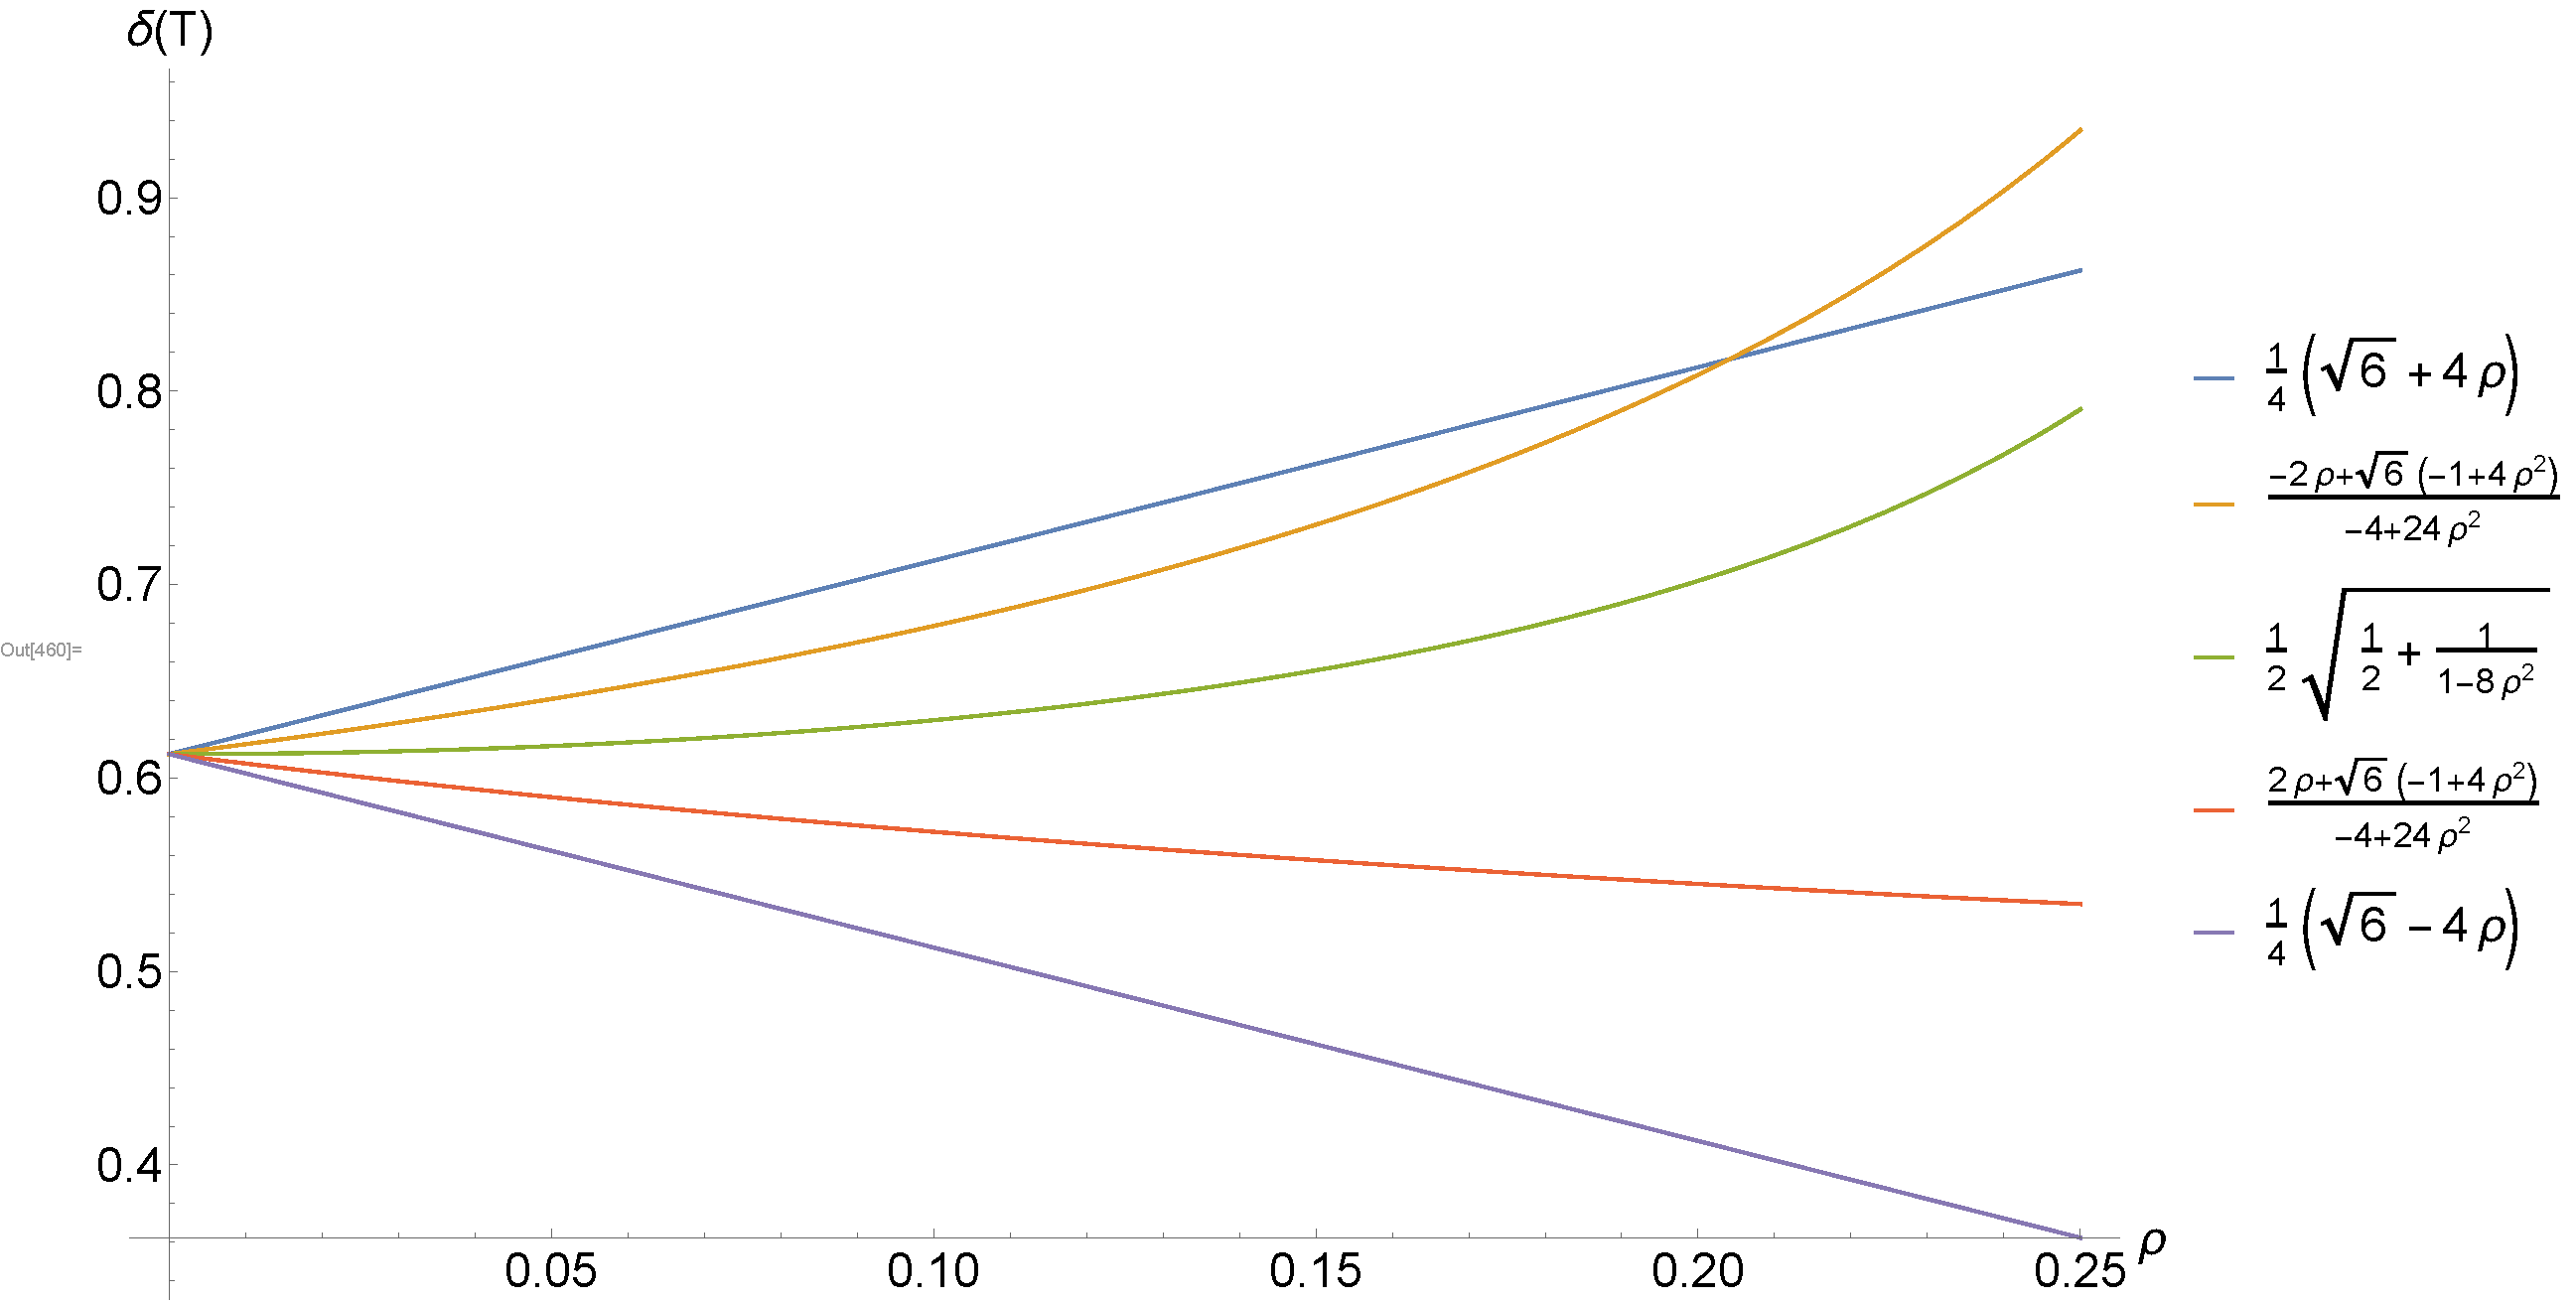
\includegraphics[height = 6cm]{./FigureLayout/t1.pdf}
\end{center}

$\delta(T)$ - circumdiameter of the tetrahedron \newline
$\rho$ - radius of the sphere in which the points can move








\end{frame}






%%%%% =====================================================================================
\begin{frame}[noframenumbering]\frametitle{References}
	
	\begin{enumerate}
		\item \textit{D. Dereudre and F. Lavancier. Practical simulation and estimation for
Gibbs Delaunay-Voronoi tessellations with geometric hardcore interaction.
Computational Statistics and Data Analysis, 55(1):498-519, 2011.}

\item \textit{D. Dereudre, R. Drouilhet, and H.O. Georgii. Existence of gibbsian point
processes with geometry-dependent interactions. Probability Theory and
Related Fields, 153(3):643-670, 2012}


\item \textit{Fropuff. The vertex configuration of a tetrahedral-octahedral honeycomb., 2006.
	URL https://en.wikipedia.org/wiki/File:TetraOctaHoneycomb-VertexConfig.svg}
\end{enumerate}

\end{frame}



%%%%% =====================================================================================



\end{document}
